%% LyX 2.1.2.2 created this file.  For more info, see http://www.lyx.org/.
%% Do not edit unless you really know what you are doing.
\documentclass[english]{sig-alternate-2013}
\usepackage[T1]{fontenc}
\usepackage[latin9]{inputenc}
\usepackage{color}
\usepackage{array}
\usepackage{verbatim}
\usepackage{graphicx}
\PassOptionsToPackage{normalem}{ulem}
\usepackage{ulem}

\makeatletter

%%%%%%%%%%%%%%%%%%%%%%%%%%%%%% LyX specific LaTeX commands.
%% Because html converters don't know tabularnewline
\providecommand{\tabularnewline}{\\}

%%%%%%%%%%%%%%%%%%%%%%%%%%%%%% User specified LaTeX commands.
\usepackage{subfigure}
\usepackage{algorithmic}
\DeclareMathOperator*{\argmax}{arg\,max}

\newcommand{\subfour}[1]{\vspace*{3mm}{\noindent\bf #1}}

\permission{Permission to make digital or hard copies of all or part of this work for personal or classroom use is granted without fee provided that copies are not made or distributed for profit or commercial advantage and that copies bear this notice and the full citation on the first page. Copyrights for components of this work owned by others than ACM must be honored. Abstracting with credit is permitted. To copy otherwise, or republish, to post on servers or to redistribute to lists, requires prior specific permission and/or a fee. Request permissions from Permissions@acm.org.}
\conferenceinfo{ICAIL '15,}{June 08 - 12, 2015, San Diego, CA, USA .} 

\CopyrightYear{2015} 
\crdata{978-1-4503-3522-5/15/06} 
\clubpenalty=10000 
\widowpenalty = 10000

\makeatother

\usepackage{babel}
\begin{document}
%\title{An Evaluation of Query Expansion for Patent Prior Art Search}
%\title{Query Expansion Methods for Patent Prior Art Search with Partial Applications}
%\title{Query Expansion Methods for Prior Art Search with Partial Patent Applications}
\title{A Study of Query Reformulation for Patent Prior Art Search with Partial Patent Applications}
%\title{ A Study of Query Reformulation for Patent Prior Art Search}
\numberofauthors{1}
\author{
%Contribution ID: 5
\alignauthor
Mohamed Reda Bouadjenek$^{\dag}$\titlenote{This work has been mainly done when the authors was at NICTA, Canberra, Australia.}, Scott Sanner$^{\Large \ddag \footnotemark[1]}$  , Gabriela Ferraro$^\S$\\
$^{\dag}$\affaddr{INRIA \& LIRMM University of Montpellier France, reda.bouadjenek@inria.fr}\\
$^{\ddag}$\affaddr{Oregon State University, Corvallis, OR 97331 USA, ssanner@gmail.com}\\
		$^\S$\affaddr{NICTA, Australian National University,  gabriela.ferraro@nicta.com.au}
%Reda Bouadjenek\titlenote{This work has been mainly done when the authors was at NICTA, Canberra, Australia.}\\
%       \affaddr{INRIA \& LIRMM}\\
%		\affaddr{Montpellier, France}\\
%       \email{reda.bouadjenek@inria.fr}
%\alignauthor
%Scott Sanner$^{\Large \footnotemark[1]}$\\
%       \affaddr{Oregon State University}\\
%		\affaddr{Corvallis, USA}\\
%       \email{ssanner@gmail.com}
%\alignauthor
%Gabriela Ferraro\\
%       \affaddr{NICTA \& ANU}\\
%		\affaddr{Canberra, Australia}\\
%       \email{gabriela.ferraro@nicta.com.au}
}
\newtheorem{proposition}{Proposition}
\maketitle

\begin{abstract}
Patents are used by legal entities to legally protect their inventions
and represent a multi-billion dollar industry of licensing and litigation.
In 2013, 302,948 patent applications were approved in the US alone
-- a number that has doubled in the past 15 years and which makes
prior art search a daunting, but necessary task in the patent application
process. In this work, we seek to investigate the efficacy of prior
art search strategies from the perspective of the inventor who wishes
to assess the patentability of their ideas prior to writing a full
application. While much of the literature inspired by the evaluation
framework of the CLEF-IP competition has aimed to assist patent examiners
in assessing prior art for complete patent applications, less of this
work has focused on patent search with queries representing partial
applications. In the (partial) patent search setting, a query is often
much longer than in other standard IR tasks, e.g., the description
section may contain hundreds or even thousands of words. While the
length of such queries may suggest query reduction strategies to remove
irrelevant terms, intentional obfuscation and general language used
in patents suggests that it may help to expand queries with additionally
relevant terms. To assess the trade-offs among all of these pre-application
prior art search strategies, we comparatively evaluate a variety of
partial application search and query reformulation methods. Among
numerous findings, querying with a full description, perhaps in conjunction
with generic (non-patent specific) query reduction methods, is recommended
for best performance. However, we also find that querying with an
abstract represents the best trade-off in terms of writing effort
vs. retrieval efficacy (i.e., querying with the description sections
only lead to marginal improvements) and that for such relatively short
queries, generic query expansion methods help. 

%This has led the research to focus on query%reformulation for patent search.  In this paper, we carry out an%intensive study of both patent-specific and standard query%reformulation methods for patent prior art search with partial patent%applications.  We found that query expansion methods are useful for%short queries (title, abstract and claims), and query reduction%methods are often useful for medium-length sections (abstract and claims).%We also shown that the abstract is a good section to query with,%suggesting that writing the abstract is useful in the early stages of%a patent drafting.

%We intend to mainly answer the following questions: \emph{What are these query reformulation methods? How do they work? What is the best section in a patent application to use as a query? What is the best query reformulation method? }
\end{abstract}

\vspace{1mm}
\noindent
{\bf Categories and Subject Descriptors:} H.3.3 {[Information Systems]}: {Information Search and Retrieval}

\vspace{1mm}
\noindent
{\bf General Terms:} Algorithms, Experimentation.

\vspace{1mm}
\noindent
{\bf Keywords:} Query Reformulation, Patent Search. 


\section{Introduction}

\noindent Patents are used by legal entities to legally protect their
inventions and represent a multi-billion dollar industry of licensing
and litigation. In 2013, 302,948 patent applications were approved
in the US alone%
\footnote{\texttt{http://www.uspto.gov/web/offices/ac/ido/oeip/taf/ us\_stat.htm}%
}, a number that has doubled in the past 15 years. Given that a single
existing patent may invalidate a new patent application, helping inventors
assess the patentability of an idea through a patent prior art search
before writing a complete patent application is an important task.

Patent prior art search involves finding previously granted patents
that may be relevant to a new patent application. The objective and
challenges of standard formulations of patent prior art search are
different from those of standard text and web search since \cite{Magdy2012}:
(i) queries are (partial) patent applications, which consist of documents
with hundreds or thousands of words organized into several sections,
while typical queries in text and web search constitute only a few
words; and (ii) patent prior art search is a recall-oriented task,
where the primary focus is to retrieve all relevant documents at early
ranks, in contrast to text and web search that are precision-oriented,
where the primary goal is to retrieve a subset of documents that satisfy
the query intent. Another important characteristic of patent prior
art search is that, in contrast to scientific and technical writers,
patent writers tend to generalize and maximize the scope of what is
protected\textcolor{red}{{} }by a patent and potentially discourage
further innovation by third parties, which further complicates the
task of formulating effective queries. For instance, abstract and
vague terms are sometimes pre-referred to concrete ones, e.g., recording
means vs. recording apparatus; resources vs. battery life; machines
located at point of sale locations vs. vending machines, etc.

\begin{figure}[t]
\begin{centering}
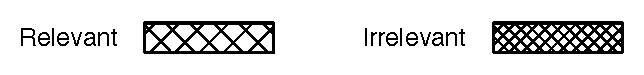
\includegraphics[width=6cm]{img/legend2} 
\par\end{centering}

\begin{centering}
\subfigure[Title query.]{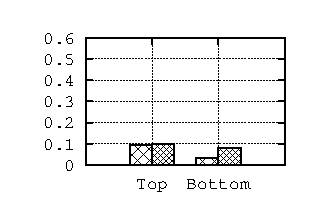
\includegraphics[width=4.2cm]{Results-CIKM2014/jaccard-qTitle-CLEF-IP2010}}\subfigure[Abstract query.]{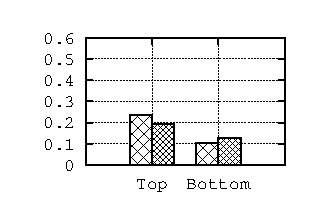
\includegraphics[width=4.2cm]{Results-CIKM2014/jaccard-qAbstract-CLEF-IP2010}}
\par\end{centering}

\begin{centering}
\subfigure[Extended Abstract]{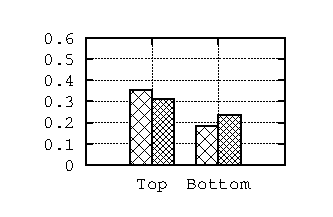
\includegraphics[width=4.2cm]{Results-CIKM2014/jaccard-qDescriptionP5-CLEF-IP2010}}\subfigure[Description query.]{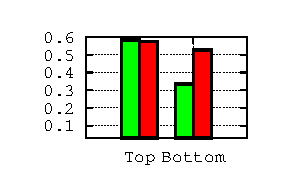
\includegraphics[width=4.2cm]{Results-CIKM2014/jaccard-qDescription-CLEF-IP2010}}
\protect\caption{Average Jaccard similarity between fields of topics and the corresponding
(ir)relevant documents for different sets of top and bottom performing
queries.}

\par\end{centering}

{\footnotesize{}{}%different queries (representing the title, abstract, or claims of a patent application)
%and the labeled (ir)relevant documents for the best (top) and worst (bottom) performing
%queries from CLEF-IP 2010 w.r.t. MAP.}
}\label{fig:FailureAnalysis} 
\end{figure}


While much of the literature inspired by the evaluation framework
of the CLEF-IP competition has aimed to assist patent examiners in
assessing prior art for complete patent applications, less work has
focused on assessing the patentability of inventions before writing
a full patent application. Furthermore, prior art search with queries
that represent unfinished patent applications is generally desirable,
since writing a full application is time-consuming and costly, especially
if lawyers are hired to assist. Hence, in this paper we consider only
sections which are more likely to be written by the inventor (or a
patent attorney) at an early stage of a patent drafting, namely: (1)
the title, (2) the abstract, (3) the description section, and (4)
an extended abstract, which we consider as the 5 first paragraphs
of the description section. However, we consider that the claims section
is more likely to be written by a patent attorney at the final stage
of a patent application.

%However prior art search with partial applications is much different than queries with a full application -- namely because the queries are much shorter and represent only parts of a patent application.

%NOTE: start a paragaph with the key idea%A patent application is organized in, at least, four sections: title,%abstract, claims and description. We assumed that a partial application%consist in one of the mentioned sections. 

To assess the difficulty of querying with partial patent applications,
we refer to Figure \ref{fig:FailureAnalysis}. Here we show an analysis
of the average Jaccard similarity%
\footnote{The Jaccard similarity is used to measure the term overlap between
two sets. Before applying the Jaccard similarity, patent-specific
stop-words were removed, as suggested by \cite{Mahdabi2012}.%
} between different queries (representing the title, abstract, the
extended abstract or descriptions of partial patent applications)
and the labeled relevant (all) and irrelevant documents (top 10 irrelevant
documents ranked by BM25 \cite{Robertson1993}). We show results for
the top 100 and bottom 100 queries (100 queries that perform the best,
and 100 queries that perform the worst) of CLEP-IP 2010 evaluated
according to Mean Average Precision (MAP). Note that while the title
section is usually composed of an average of six terms, the other
sections are longer, ranging from ten to thousands of terms. There
are three notable trends here: (i) term overlap increases from title
to description since the query size grows accordingly; (ii) the bottom
100 performing queries tend to have much smaller term overlap with
the relevant documents than the top 100 queries; and (iii) even in
the best case of querying with very long description sections, the
average term overlap indicates many terms of relevant documents are
not found in the query.

%**Highly redundant with above content**%While these results suggest the description section is the best part%of a partial patent application to use as query, they also point out%that the term overlap between the queries and the relevant documents%can be very low. Also, in this context, a query is much longer than%in other standard IR tasks. It can take the form of a long paragraph%(e.g. the case of the abstract used for querying), or even a very%long document (e.g. the case of claims or the description used for%querying). 

Similar observations in the general patent prior art search literature
\cite{Magdy2011} have led to a research focus on query reformulation.
Therefore, we suggest an investigation of \emph{query reformulation}
\cite{Baeza-Yates2010} methods as a means for improving the term
overlap between queries that represent partial patent applications
and relevant documents, with the objective of assessing not only the
performance of standard query reformulation methods, but also the
effectiveness of query reformulation methods that exploit patent-specific
characteristics.

In summary, to aid the patent inventor in developing an effective
pre-application prior art search strategy, we seek to answer the following
questions: %in this work: 
\begin{itemize}
\item What parts of a patent application should a patent inventor or a patent
attorney write first to achieve effective prior art search? What are
the trade-offs in section writing effort vs. the retrieval performance
of querying with that section? We assume the writing effort to be
a function of word number. 
\item In query expansion, which patent section is the best source for term
expansion? %do any sections of patents serve as better sources of expansion terms?  Which expansion methods work best, and in which settings? 
\item For query reformulation (both query expansion and reduction), which
methods work best, and in which settings? Do patent-specific reformulation
methods offer advantages over more generic IR reformulation methods? 
\end{itemize}
To answer these questions, we perform a thorough comparative analysis
of partial patent application query strategies and reformulation methods
on the CLEF-IP patent prior art search datasets.

The rest of the paper is organized as follows: in Section \ref{sec:QueryReformulation},
we present a variety of generic and patent-specific query reformulation
methods; in Section \ref{sec:Evaluation}, we present the evaluation
results and analysis to answer the above questions; in Section \ref{sec:RelatedWork}
we discuss the related work on other patent-specific query reformulation
methods, which are not considered in this paper; and in Section \ref{sec:Conclusion},
we conclude with key observations from the evaluation that lead to
concrete recommendations for patent prior art search with partial
applications.


\section{Query Reformulation for Patents}

\label{sec:QueryReformulation}

Query Reformulation is the process of transforming an initial query
$Q$ to another query $Q'$. This transformation may be either an
expansion or a reduction of the query.\emph{ Query Expansion} (QE)
\cite{Baeza-Yates2010} enhances the query with additional terms likely
to occur in relevant documents. Hence, given a query representation
$Q$, QE aims to select an optimal subset $T_{k}$ of $k$ terms,
which are relevant to $Q$, then build $Q'$ such as $Q'=Q\cup T_{k}$.
As for \emph{Query Reduction} (QR) \cite{Kumaran2009}, it is the
process that reduces the query such that superfluous information is
removed. Hence, given a query representation $Q$, QR aims to select
an optimal subset $T_{k}\subset Q$ of $k$ terms, which are relevant
to $Q$, then build $Q'$ such as $Q'=T_{k}$.

The outline of the following subsections is as follows: Section \ref{sec:UtilityQR}
motivates query reduction for patent prior art search. Then, we describe
the standard and patent-specific query reformulation methods that
we evaluate in Section \ref{sec:Evaluation}.

%In the following subsections, we first give a motivation behind using query reduction for patent search in Section \ref{sec:UtilityQR}.


\subsection{Utility of Query Reduction for Patents}

\label{sec:UtilityQR}

While the title is usually composed by an average of six terms, the
other sections are longer, ranging from ten to thousands of terms.
Therefore, we investigate the impact of query reduction methods only
when querying with long sections such as abstract, extended abstract
or description.

Table \ref{tbl:queryPAC-1019} provides insight into the utility of
query reduction for the abstract section of the Topic PAC-1019%
\footnote{\texttt{http://www.lens.org/lens/patent/WO\_2005\_100300\_A1}%
} from the CLEF-IP 2010 data collection. The baseline query, which
is the original query (provided in the header row) after stemming
and stop-word removal , had an Average Precision (AP) of 0.280 and
a Patent Retrieval Evaluation Score (PRES)%
\footnote{The PRES metric places more emphasis on high-recall retrieval by weighting
relevant documents lower in the ranking more highly than MAP. %
} \cite{Magdy2010a} of 0.777 (its performance are provided in the
footer row). We show the evaluation performance of the query after
removing each term from the original query. The removed terms have
been sorted in the order of decreasing PRES. We can observe that there
are ten terms (highlighted in boldface) that if they are (individually)
removed from the query, the PRES of the original long query increased.

\begin{table}[t]
\begin{centering}
\protect\caption{Sample of terms removed from the abstract section of CLEP-IP2010 Topic
PAC-1019. }
{\footnotesize{}\label{tbl:queryPAC-1019}} 
\par\end{centering}

\centering{}{\scriptsize{}}%
\begin{tabular}{|l|c|c|c|c|c|}
\hline 
\multicolumn{6}{|>{\raggedright}p{8cm}|}{\textbf{\scriptsize{}Topic:}{\scriptsize{} PAC-1019 (Doc num: WO2005100300
A1)}}\tabularnewline
\hline 
\multicolumn{6}{|>{\raggedright}p{8cm}|}{\textbf{\scriptsize{}Abstract:}{\scriptsize{} A 5-aminolevulinic acid
salt which is useful in fields of microorganisms, fermentation, animals,
medicaments, plants and the like; a process for producing the same;
a medical composition comprising the same; and a plant activator composition
comprising the same.}}\tabularnewline
\hline 
\hline 
\textbf{\scriptsize{}Term removed} & \textbf{\scriptsize{}P@5} & \textbf{\scriptsize{}P@10} & \textbf{\scriptsize{}R@10} & \textbf{\scriptsize{}AP} & \textbf{\scriptsize{}PRES}\tabularnewline
\hline 
\textbf{\scriptsize{}composit...} & \textbf{\scriptsize{}0.600} & {\scriptsize{}0.300} & {\scriptsize{}0.428} & \textbf{\scriptsize{}0.360} & \textbf{\scriptsize{}0.829}\tabularnewline
\hline 
\textbf{\scriptsize{}activ...} & {\scriptsize{}0.400} & {\scriptsize{}0.300} & {\scriptsize{}0.428} & {\scriptsize{}0.277} & \textbf{\scriptsize{}0.809}\tabularnewline
\hline 
\textbf{\scriptsize{}anim...} & \textbf{\scriptsize{}0.600} & {\scriptsize{}0.300} & {\scriptsize{}0.428} & \textbf{\scriptsize{}0.345} & \textbf{\scriptsize{}0.798}\tabularnewline
\hline 
\textbf{\scriptsize{}produc...} & {\scriptsize{}0.400} & {\scriptsize{}0.300} & {\scriptsize{}0.428} & \textbf{\scriptsize{}0.286} & \textbf{\scriptsize{}0.797}\tabularnewline
\hline 
\textbf{\scriptsize{}ferment...} & {\scriptsize{}0.200} & {\scriptsize{}0.300} & {\scriptsize{}0.428} & \textbf{\scriptsize{}0.283} & \textbf{\scriptsize{}0.796}\tabularnewline
\hline 
\textbf{\scriptsize{}microorgan...} & \textbf{\scriptsize{}0.600} & {\scriptsize{}0.300} & {\scriptsize{}0.428} & \textbf{\scriptsize{}0.333} & \textbf{\scriptsize{}0.793}\tabularnewline
\hline 
\textbf{\scriptsize{}compris...} & {\scriptsize{}0.400} & {\scriptsize{}0.300} & {\scriptsize{}0.428} & {\scriptsize{}0.271} & \textbf{\scriptsize{}0.790}\tabularnewline
\hline 
\textbf{\scriptsize{}medica...} & {\scriptsize{}0.400} & {\scriptsize{}0.300} & {\scriptsize{}0.428} & \textbf{\scriptsize{}0.297} & \textbf{\scriptsize{}0.789}\tabularnewline
\hline 
\textbf{\scriptsize{}field...} & {\scriptsize{}0.400} & {\scriptsize{}0.300} & {\scriptsize{}0.428} & \textbf{\scriptsize{}0.282} & \textbf{\scriptsize{}0.782}\tabularnewline
\hline 
{\scriptsize{}plant...} & {\scriptsize{}0.200} & {\scriptsize{}0.200} & {\scriptsize{}0.285} & {\scriptsize{}0.114} & {\scriptsize{}0.774}\tabularnewline
\hline 
{\scriptsize{}process...} & {\scriptsize{}0.400} & {\scriptsize{}0.300} & {\scriptsize{}0.428} & {\scriptsize{}0.279} & {\scriptsize{}0.764}\tabularnewline
\hline 
{\scriptsize{}acid...} & {\scriptsize{}0.400} & {\scriptsize{}0.300} & {\scriptsize{}0.428} & {\scriptsize{}0.252} & {\scriptsize{}0.693}\tabularnewline
\hline 
{\scriptsize{}salt...} & {\scriptsize{}0.200} & {\scriptsize{}0.200} & {\scriptsize{}0.285} & {\scriptsize{}0.216} & {\scriptsize{}0.663}\tabularnewline
\hline 
{\scriptsize{}aminolevulin...} & {\scriptsize{}0.000} & {\scriptsize{}0.100} & {\scriptsize{}0.142} & {\scriptsize{}0.026} & {\scriptsize{}0.352}\tabularnewline
\hline 
\hline 
\textbf{\scriptsize{}Baseline} & {\scriptsize{}0.400} & {\scriptsize{}0.300} & {\scriptsize{}0.428} & {\scriptsize{}0.280} & {\scriptsize{}0.777}\tabularnewline
\hline 
\end{tabular}
\end{table}


Figure \ref{fig:QRUtility} shows the summary upper-bound performance
for precision, recall, MAP, Mean Reciprocal Rank (MRR), and PRES that
can be achieved for a set of 1304 abstract queries from the CLEF-IP
2010 data collection. ``Baseline\textquotedblright{} refers to a
probabilistic BM25 retrieval model \cite{Robertson1993} run using
the Lucene search engine \cite{McCandless2010} and the original long
query. ``Oracle\textquotedblright{} refers to the situation where
all terms with negative impact are removed from the original long
query following the previous process. This gives us an upper bound
on the performance that can be realized through query reduction for
this set of queries. It is this statistically significant improvement
in performance through query reduction that we can target for the
abstract and the description sections.

\begin{figure}[!h]
\centering{}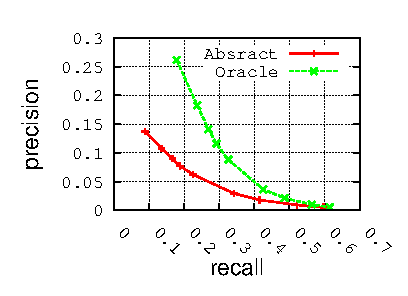
\includegraphics[width=4.3cm]{analysis/precision-recall_ByField-CLEF-IP_2010}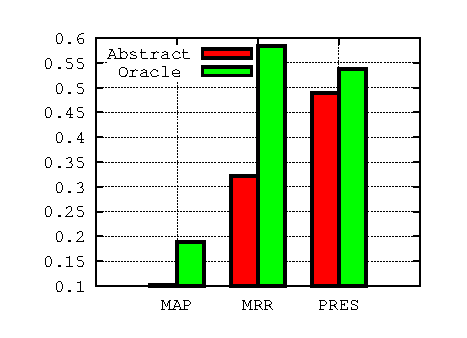
\includegraphics[width=4.3cm]{analysis/MAP-MRR_ByField-CLEF-IP_2010}
\protect\caption{The utility of query reduction for 1304 abstract queries of the CLEF-IP
2010 dataset. }
{\footnotesize{}\label{fig:QRUtility}}
\end{figure}



\subsection{Generic Query Reformulation Methods}

\label{sec:StandardQRMethods}

\subfour{The Rocchio Algorithm for Relevance Feedback:} The Rocchio
algorithm \cite{Salton1971} is a classic algorithm of relevance feedback
used mainly for query expansion. In brief, it provides a method of
incorporating relevance feedback information into the vector space
model representing a query \cite{Manning2008}. The underlying theory
behind Rocchio is to find a query vector $\overrightarrow{Q'}$, that
maximizes similarity with relevant documents while minimizing similarity
with irrelevant documents. Typically, a pseudo-relevance feedback
(PRF) set of $k$ top ranked documents obtained after an initial run
of the query is considered as the set of relevant documents to build
$\overrightarrow{Q'}$. We refer to this method as RocchioQE%
\footnote{We used the LucQE module, which provides an implementation of the
Rocchio method for Lucene.\\ \texttt{http://lucene-qe.sourceforge.net/}%
}.

Similarly, Rocchio can be used as a QR method. Basically, the idea
is that once the Rocchio-modified query vector has been computed,
it is possible to select only the terms that appear in the initial
query $Q$ and rank them using the Rocchio score and finally, select
the top $k$ terms with the highest score to build $Q'$. We refer
to this approach as RocchioQR.

\subfour{Maximal Marginal Relevance for Query Reformulation:} As
a general method for query reformulation, we also consider a method
of ``diverse'' term selection --- an adaptation of the \emph{Maximal
Marginal Relevance} (MMR) \cite{Carbonell1998} algorithm for result
set diversification. But, rather than use MMR for diverse document
selection (as typically used), it is used here for diverse term selection
--- the hypothesis being that diverse term selection may improve coverage
of relevant terms in the PRF set.

%The idea is to use MMR for diverse term selection. %\subfour{MMR Query Expansion (MMRQE)}%\label{sec:MMRQE}

%%%%%%%%%%%%%%%%%%%%%%%%%%%%%%%%%%%%%%%%%%%%%%%%%%%%%%%%%%%%%%%%%%%%%
\begin{figure}[!t]
\begin{centering}
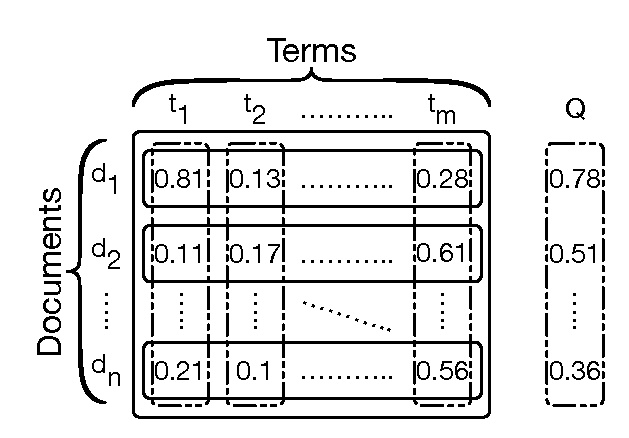
\includegraphics[width=5cm]{img/matrix} 
\par\end{centering}

\protect\protect\caption{Notation used in MMR QE/QR.}


\label{fig:Notation} 
\end{figure}


%%%%%%%%%%%%%%%%%%%%%%%%%%%%%%%%%%%%%%%%%%%%%%%%%%%%%%%%%%%%%%%%%%%%%

In the case of QE, we call this diversified expansion method MMR Query
Expansion (MMRQE). MMRQE takes as input a PRF set, which is used to
build a document-term matrix of $n$ documents and $m$ terms as shown
in Figure \ref{fig:Notation} (the TF-IDF is used to populate the
matrix for each document vector). To represent the query $Q$ in the
documents' dimension as in Figure \ref{fig:Notation}, we use the
BM25 or TF-IDF score between each document $d_{i}$ and the query.
Hence, given a query representation $Q$, MMRQE aims to select an
optimal subset of $k$ terms $T_{k}^{*}\subset D$ (where $|T_{k}^{*}|=k$
and $k\ll|m|$, and $D$ is the PRF set) relevant to $Q$ but inherently
different from each other (i.e., diverse). This can be achieved by
building $T_{k}^{*}$ in a greedy manner by choosing the next optimal
term $t_{k}^{*}$ given the previous set of optimal term selections
$T_{k-1}^{*}=\{t_{1}^{*},\ldots,t_{k-1}^{*}\}$ (assuming $T_{0}^{*}=\emptyset$)
using the MMR diverse selection criterion:

\begin{equation}
t_{k}^{*}=\argmax_{t_{k}\notin T_{k-1}^{*}}\hspace{-0.3mm}[\lambda\cos(Q,t_{k})-\hspace{-0.3mm}(1-\lambda)\max_{t_{j}\in T_{k-1}^{*}}\cos(t_{j},t_{k})]\label{eq:MMRQE-QR}
\end{equation}


\noindent Here, the first cosine similarity term measures relevance
between the query $Q$ and possible expansion term $t_{k}$ while
the second term penalizes the possible expansion term according to
its cosine similarity with any currently selected term in $T_{k-1}^{*}$.
Note that these similarities are computed based on vectors extracted
from the PRF set as illustrated in Figure \ref{fig:Notation}. The
parameter $\lambda\in[0,1]$ trades off relevance and diversity. For
MMRQE, we found that $\lambda=0.5$ generally provides the best results,
according to our experiments on the CLEF-IP training dataset collection.

For QR, we can greedily rebuild the query from scratch, while choosing
diversified terms from the query itself. Here, we call this approach
MMR Query Reduction (MMRQR). Formally, given a query representation
$Q$, MMRQR aims to select an optimal subset of $k$ terms $T_{k}^{*}\subset Q$
(where $|T_{k}^{*}|=k$ and $k<|Q|$) relevant to $Q$ but inherently
different from each other (i.e., diverse). This can be achieved by
building $T_{k}^{*}$ in a greedy manner by choosing the next optimal
term $t_{k}^{*}$ given the previous set of optimal term selections
$T_{k-1}^{*}=\{t_{1}^{*},\ldots,t_{k-1}^{*}\}$ (assuming $T_{0}^{*}=\emptyset$)
using an adaptation of the MMR diverse selection criterion. Note that
we use all the sections of the patent documents in the PRF set to
built the document-term matrix of $n$ documents and $m$ terms shown
in Figure \ref{fig:Notation}. For MMRQR, we found that $\lambda=0.8$
generally provide the best results in our experiments on the CLEF-IP
dataset collection.

The key insight we want to highlight is that MMRQE does not select
expansion terms independently as in practical usage of Rocchio, but
rather it selects terms that have uncorrelated usage patterns across
documents, thus hopefully encouraging diverse term selection that
covers more documents for a fixed expansion budget $k$ and ideally,
higher recall.


\subsection{Patent-specific Query Reformulation Methods}

\label{sec:SpecificQRMethods}

%In this section, we first describe two patent-specific query expansionmethods, then, we describe two patent-specific query reduction methods.

\subfour{Synonym Sets for Patent Query Expansion:} Magdy et al.
\cite{Magdy2011} proposed a patent query expansion method, which
automatically generates candidate synonym sets (SynSet) for terms
to use as a source of expansion terms. The idea for generating the
SynSet comes from the characteristics of the CLEF-IP patent collection,
where some of the sections in some patents are translated into three
languages (English, French, and German). They used these parallel
manual translations to create possible synonyms sets. Hence, for a
word $w$ in one language which has possible translations to a set
of words in another language ${w_{1},w_{2},\ldots,w_{n}}$, this set
of words can be considered as synonyms or at least related to each
other. The generated SynSet is used for query expansion in two ways:
(i) The first one used the probability associated with the SynSet
entries as a weight for each expanded term in the query (denoted WSynSet).
Therefore, each term was replaced with its SynSet entries with the
probability of each item in the SynSet acting as a weight to the term
within the query. (ii) The second one neglected this associated probability
and used uniform weighting for all synonyms of a given term (denoted
USynSet).

\subfour{Patent Lexicon for Query Expansion:} Mahdabi et al. \cite{Mahdabi2013}
proposed to build a query-specific patent lexicon based on definitions
of the International Patent Classification (IPC). The lexicon is simply
built by removing general and patent-specific stop-words from the
text of IPC definition pages. Each entry in the lexicon is composed
of a key and a value. The key is an IPC class and the value is a set
of terms representing the mentioned class. Then, the lexicon is used
to extract expansion concepts related to the context of the information
need of a given query patent. To this end, the IPC class of the query
patent is searched in the lexicon and the terms matching this class
are considered as candidate expansion terms. The proposed approach
tries to combine these two complementary vocabularies (i.e. terms
of the query and the IPC codes). Note that all the levels of the IPC
codes are used to build the lexicon. In this paper we refer to this
patent query expansion method as IPC Codes.

\subfour{Language Model for Query Reduction:} In \cite{Ganguly2011},
the authors proposed a query reduction technique, which decomposes
a query (a patent section) into constituent text segments and computes
Language Model (LM) similarities by calculating the probability of
generating each segment from the top ranked documents (PRF set). Then,
the query is reduced by removing the least similar segments from the
query. We refer to this method as LMQR.

\subfour{IPC Codes for Query Reduction:} Based on the intuition
that, terms in the IPC code definition may represent \textquotedbl{}stop-words\textquotedbl{}
(especially if they are infrequent in the patent application, but
appear in many documents sharing the same IPC code), a query can be
reduced as follows: %one can think to reduce a patent query as follows:
(i) For each patent application, take the definitions of the IPC codes
which are associated to it. Then, (ii) rank the terms of the query
according to the difference in their frequency in the query and their
frequency in the class code definition. Finally, (iii) remove bottom
terms of this ranking from the query (i.e. good terms are terms that
occur a lot in the query, and few in the class code definition, whereas
bad terms are those that occur few in the query, and a lot in documents
sharing the same IPC code). In the evaluation section we denote this
approach IPC-StopWords.

%%%% Reviewers may point out that we should have compared...%%


\section{Experimental Evaluation}

\label{sec:Evaluation}

In this section we first explain the experimental setup for evaluating
the effectiveness of patent prior art search with partial applications.
Then, we discuss the results of QE and QR methods in Sections \ref{sec:QEResults}
and \ref{sec:QRResults} respectively.


\subsection{Experimental Setup}

\label{sec:Setup}

For our experiments, we used used the Lucene IR System%
\footnote{\texttt{http://lucene.apache.org/}%
} to index the English subset of CLEF-IP 2010 and CLEF-IP 2011 datasets%
\footnote{\texttt{http://www.ifs.tuwien.ac.at/\textasciitilde{}clef-ip/}%
} \cite{Piroi2011,Roda2009} with the default settings for stemming
and stop-word removal. We also removed patent-specific stop-words
as described in \cite{Magdy2012}. CLEF-IP 2010 contains 2.6 million
patent documents, and the English test sets of CLEF-IP 2010 correspond
to 1303 topic sources of partial patent application queries. We also
experimented with the CLEF-IP 2011 dataset.

In our implementation, each section of a patent (title, abstract,
claims, and description) is indexed in a separate field so that different
sections can be used, for example, as source of expansion terms. However,
when a query is processed, all indexed fields are targeted, since
this generally offers best retrieval performance. %
\begin{comment}
As suggested in previous work \cite{Lopez2009,Roda2009} and found
to yield best results in our experiments, we used the patent classification
(IPC) codes assigned to the query topics to filter search results
to match at least one of the query IPC codes. 
\end{comment}
{} We report both MAP and PRES on the top 1000 results.


\subsection{Query Expansion Results}

\label{sec:QEResults}

In this section, we discuss the results of partial patent queries
with the QE methods described in Section \ref{sec:QueryReformulation}.
The configuration options and associated questions that were considered
are the following: %In doing this experimentation, there are many configuration options and associated questions to consider:
\begin{itemize}
\item \textbf{Partial patent query type:} We consider a query of a partial
patent application to consist of either the title, the abstract, the
extended abstract or the full description section. Recall that we
do not consider the Claim section, since it is more likely to be written
by a lawyer than the inventor at the final stage of a patent application.
Hence, critical questions are: what part of a partial application
an inventor should write to obtain the best search results? And what
QE methods work best for each type of query? 
\item \textbf{Query expansion source:} We consider the abstract, claims,
and description sections as different term sources to determine which
section offers the best source of expansion terms, e.g., are words
in the claims of particularly high value as expansion terms? We omit
the use of the title as a source of expansion terms noting that this
configuration performed poorly due to the relative sparsity of useful
expansion terms in the titles of the PRF set. 
\item \textbf{Relevance model:} For initial retrieval of documents in the
\emph{pseudo-relevant} feedback set (PRF) and subsequent re-retrieval,
there are various options for the relevance ranking model. In this
work, we explore a probabilistic approach represented by the popular
BM25 \cite{Robertson1993} algorithm, as well as a vector space model
(VSM) approach using TF-IDF weighting \cite{Salton1975}. A natural
question is which relevance model works best for query expansion for
patent prior art search? 
\item \textbf{Term selection method:} We consider the different query expansion
methods described above, i.e. RocchioQE, MMRQE, IPC Codes, WSynSet,
USynSet and ask what is the best QE method for patent search? 
\end{itemize}
\begin{figure*}
\begin{centering}
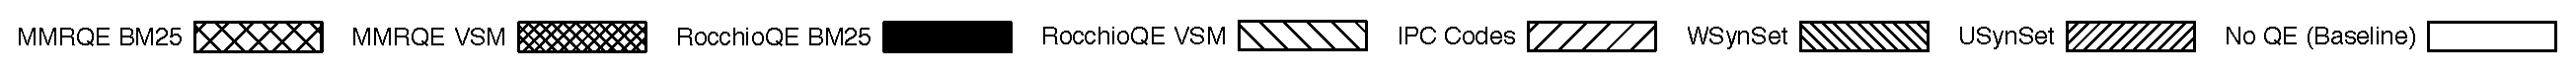
\includegraphics[width=17.5cm]{img/legendQE2} 
\par\end{centering}

\begin{centering}
\subfigure[Query Title.]{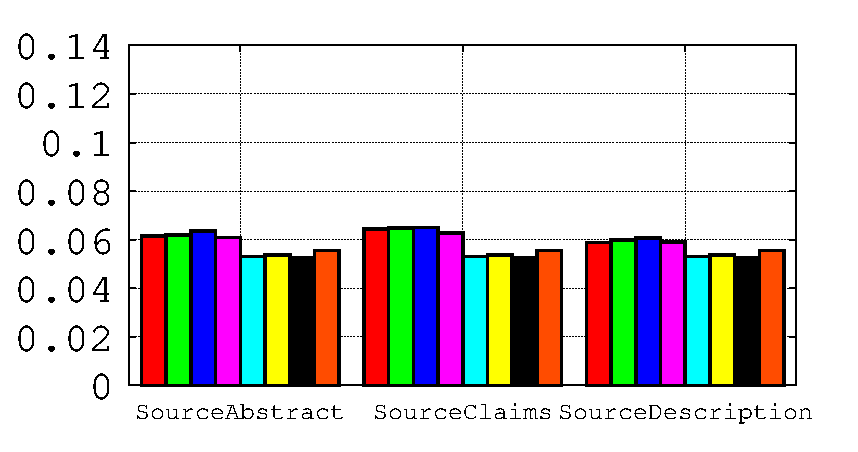
\includegraphics[width=4.5cm]{Results-CIKM2014/qTitle-MAP-CLEF-IP2010}}\subfigure[Query Abstract.]{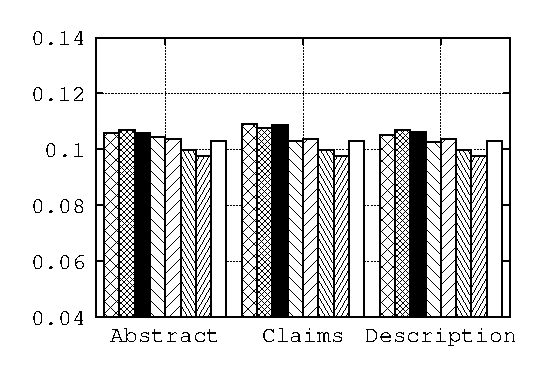
\includegraphics[width=4.5cm]{Results-CIKM2014/qAbstract-MAP-CLEF-IP2010}}\subfigure[Query Ext. Abstract.]{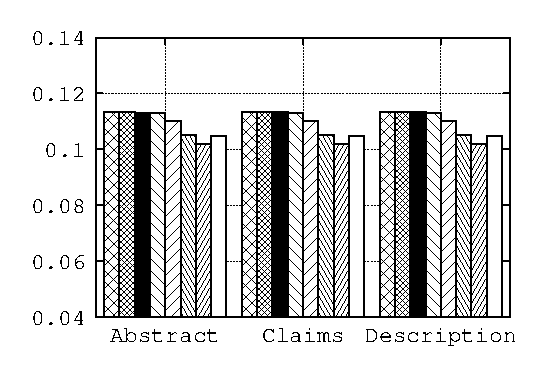
\includegraphics[width=4.5cm]{Results-CIKM2014/qExtAbstract-MAP-CLEF-IP2010}}\subfigure[Query Description.]{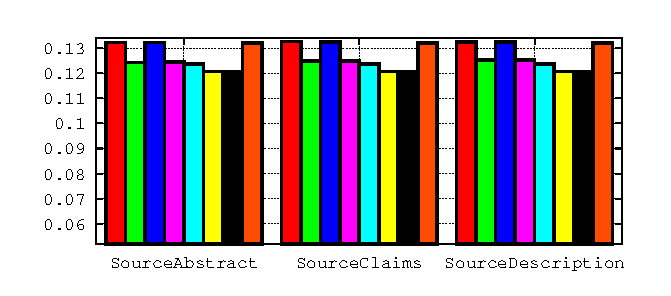
\includegraphics[width=4.5cm]{Results-CIKM2014/qDescription-MAP-CLEF-IP2010}}
\par\end{centering}

\protect\caption{MAP for QE methods on CLEF-IP 2010. The x-axis gives the query expansion
source.}


\label{fig:MAP-CLEF2010}
\end{figure*}


\begin{figure*}
\begin{centering}
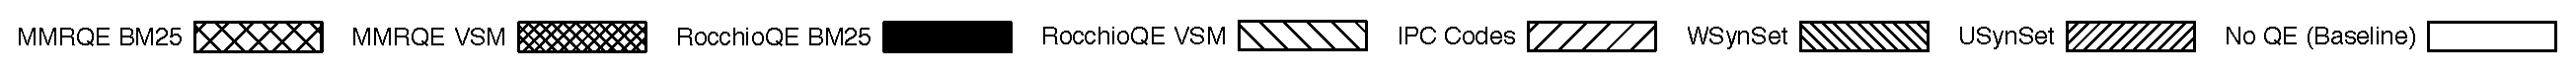
\includegraphics[width=17.5cm]{img/legendQE2}
\par\end{centering}

\begin{centering}
\subfigure[Query Title.]{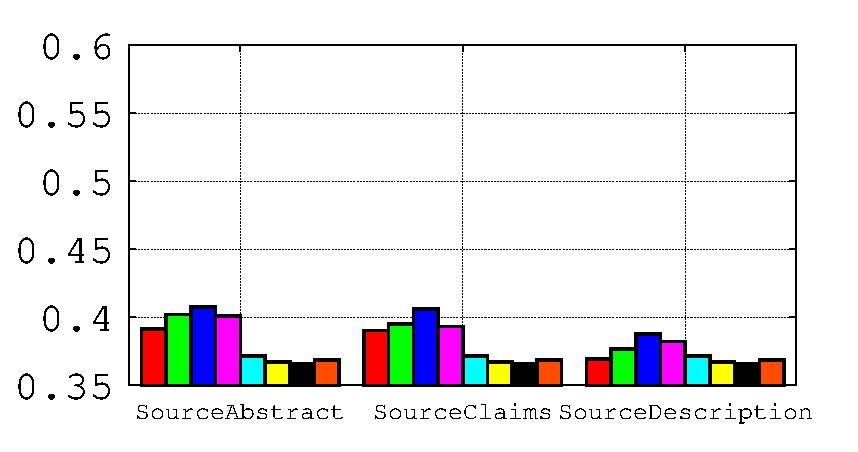
\includegraphics[width=4.5cm]{Results-CIKM2014/qTitle-PRES-CLEF-IP2010}
}\subfigure[Query Abstract.]{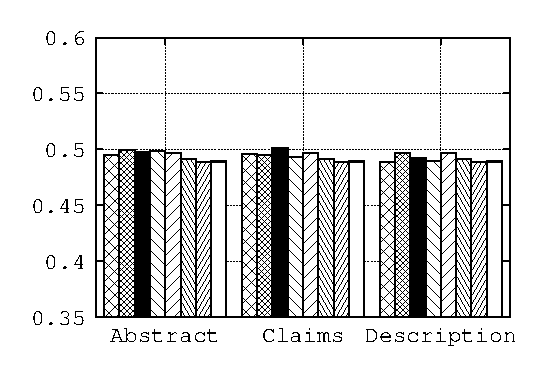
\includegraphics[width=4.5cm]{Results-CIKM2014/qAbstract-PRES-CLEF-IP2010}
}\subfigure[Query Ext. Abstract.]{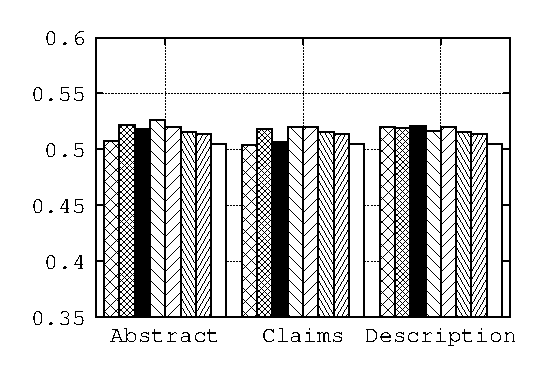
\includegraphics[width=4.5cm]{Results-CIKM2014/qExtAbstract-PRES-CLEF-IP2010}
}\subfigure[Query Description.]{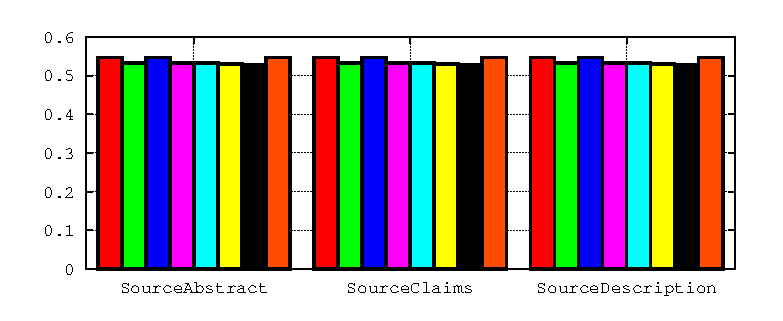
\includegraphics[width=4.5cm]{Results-CIKM2014/qDescription-PRES-CLEF-IP2010}
}
\par\end{centering}

\protect\caption{PRES for QE methods on CLEF-IP 2010. The x-axis gives the query expansion
source.}


\label{fig:PRES-CLEF2010} 
\end{figure*}


\begin{figure*}
\begin{centering}
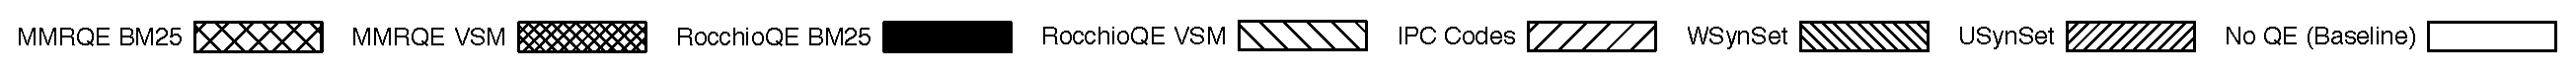
\includegraphics[width=17.5cm]{img/legendQE2}
\par\end{centering}

\begin{centering}
\subfigure[Query Title.]{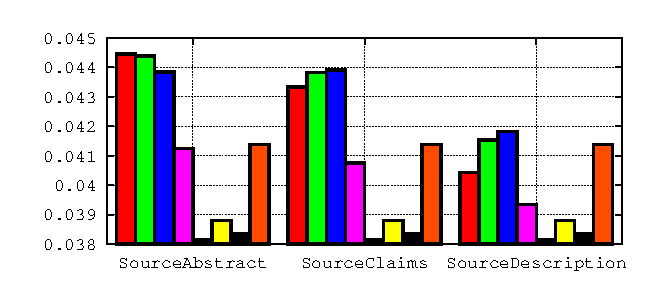
\includegraphics[width=4.5cm]{Results-CIKM2014/qTitle-MAP-CLEF-IP2011}}\subfigure[Query Abstract.]{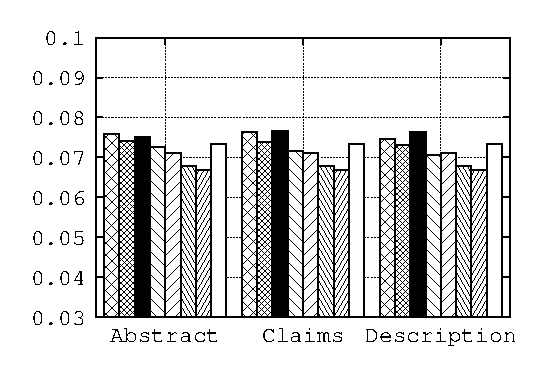
\includegraphics[width=4.5cm]{Results-CIKM2014/qAbstract-MAP-CLEF-IP2011}}\subfigure[Query Ext. Abstract.]{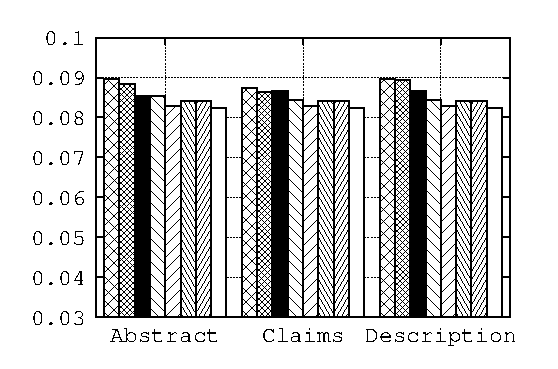
\includegraphics[width=4.5cm]{Results-CIKM2014/qExtAbstract-MAP-CLEF-IP2011}}\subfigure[Query Description.]{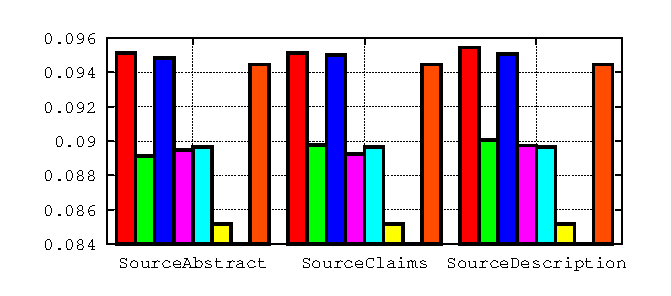
\includegraphics[width=4.5cm]{Results-CIKM2014/qDescription-MAP-CLEF-IP2011}}
\par\end{centering}

\protect\caption{MAP for QE methods on CLEF-IP 2011. The x-axis gives the query expansion
source.}


\label{fig:MAP-CLEF2011}
\end{figure*}


\begin{figure*}
\begin{centering}
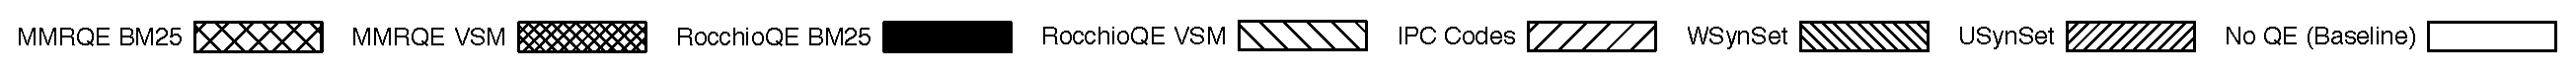
\includegraphics[width=17.5cm]{img/legendQE2}
\par\end{centering}

\begin{centering}
\subfigure[Query Title.]{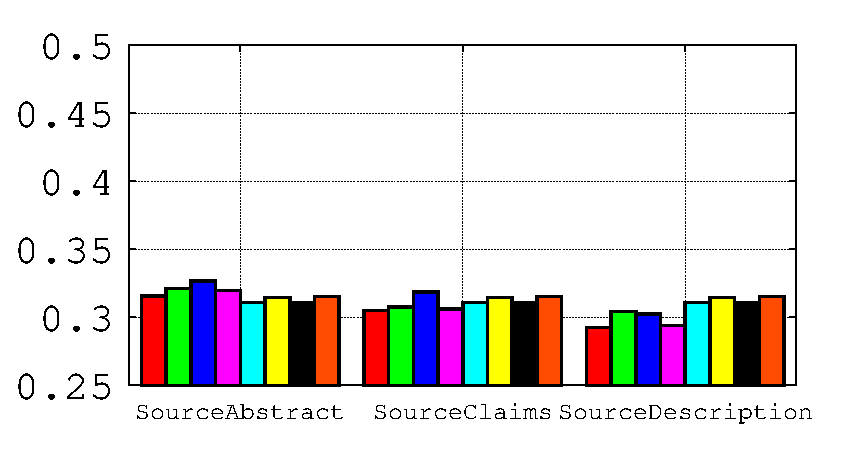
\includegraphics[width=4.5cm]{Results-CIKM2014/qTitle-PRES-CLEF-IP2011}
}\subfigure[Query Abstract.]{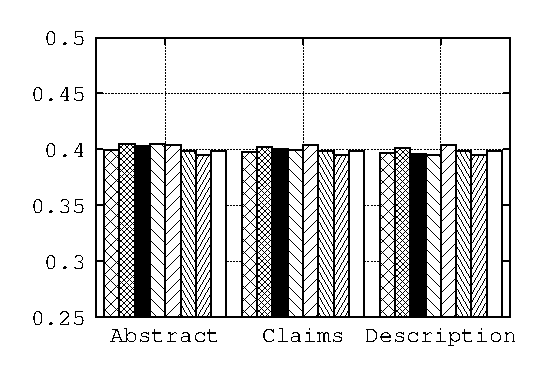
\includegraphics[width=4.5cm]{Results-CIKM2014/qAbstract-PRES-CLEF-IP2011}
}\subfigure[Query Ext. Abstract.]{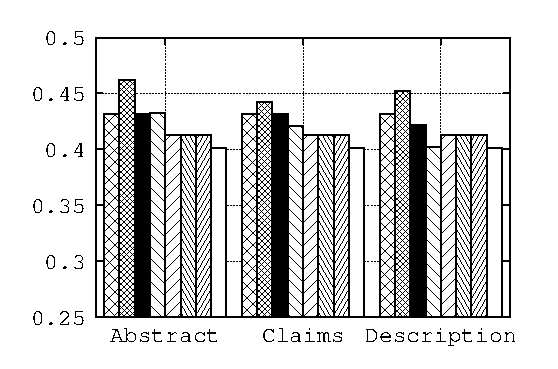
\includegraphics[width=4.5cm]{Results-CIKM2014/qExtAbstract-PRES-CLEF-IP2011}
}\subfigure[Query Description.]{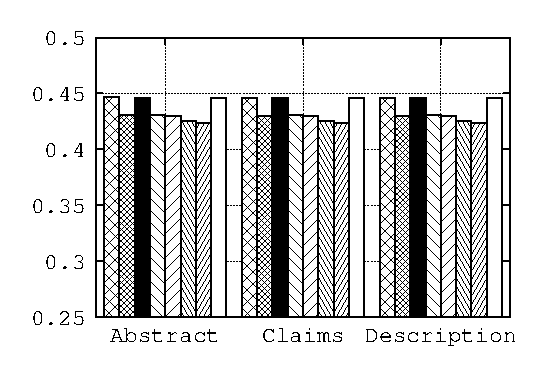
\includegraphics[width=4.5cm]{Results-CIKM2014/qDescription-PRES-CLEF-IP2011}
}
\par\end{centering}

\protect\caption{PRES for QE methods on CLEF-IP 2011. The x-axis gives the query expansion
source.}


\label{fig:PRES-CLEF2011} 
\end{figure*}


\begin{table*}[t]
\protect\caption{Samples of queries extracted from CLEF-IP 2011, where QE improves
the performance (P: Precision, R: Recall, RR: Reciprocal Rank, AP:
Average Precision, PRES: Patent Retrieval Evaluation Score). MMRQE
improves the two first examples, while Rocchio improves the third. }
\label{tbl:QESampleQueries}

\centering{}%
\begin{tabular}{|>{\raggedright}p{17.5cm}|}
\hline 
\textbf{\scriptsize{}1- Topic:}{\scriptsize{} EP-1921264-A2}\tabularnewline
\hline 
\textbf{\scriptsize{}Abstract:}{\scriptsize{} An article of manufacture
having a nominal profile substantially in accordance with Cartesian
coordinate values of X, Y and Z set forth in a TABLE 1. Wherein X
and Y are distances in inches which, when connected by smooth continuing
arcs, define airfoil profile sections at each distance Z in inches.
The profile sections at the Z distances being joined smoothly with
one another to form a complete airfoil shape (22,23).}\tabularnewline
\hline 
\begin{tabular}{>{\centering}p{16.5cm}}
{\scriptsize{}Baseline performance:}~{\scriptsize{}}%
\begin{tabular}{|c|c|c|c|c|c|c|c|c|c|c|c|}
\hline 
\textbf{\scriptsize{}P@5:} & {\scriptsize{}0.000} & \textbf{\scriptsize{}P@10:} & {\scriptsize{}0.000} & \textbf{\scriptsize{}R@10:} & {\scriptsize{}0.000} & \textbf{\scriptsize{}RR:} & {\scriptsize{}0.066} & \textbf{\scriptsize{}AP:} & {\scriptsize{}0.043} & \textbf{\scriptsize{}PRES:} & {\scriptsize{}0.777}\tabularnewline
\hline 
\end{tabular}\tabularnewline
\end{tabular}\tabularnewline
\hline 
\textbf{\scriptsize{}MMRQE expanded terms:}{\scriptsize{} }\textbf{\scriptsize{}\uline{airfoil}}{\scriptsize{},
}\textbf{\scriptsize{}rotor}{\scriptsize{}, }\textbf{\scriptsize{}blend}{\scriptsize{},
}\textbf{\scriptsize{}substanti}{\scriptsize{}, }\textbf{\scriptsize{}\uline{root}}{\scriptsize{},
}\textbf{\scriptsize{}\uline{portion}}{\scriptsize{}, }\textbf{\scriptsize{}includ}{\scriptsize{},
}\textbf{\scriptsize{}suction}{\scriptsize{}, }\textbf{\scriptsize{}\uline{form}}{\scriptsize{},
}\textbf{\scriptsize{}tip}\tabularnewline
\hline 
\begin{tabular}{>{\centering}p{16.5cm}}
{\scriptsize{}MMRQE performance:}~{\scriptsize{}}%
\begin{tabular}{|c|c|c|c|c|c|c|c|c|c|c|c|}
\hline 
\textbf{\scriptsize{}P@5:} & {\scriptsize{}0.000} & \textbf{\scriptsize{}P@10:} & {\scriptsize{}0.200} & \textbf{\scriptsize{}R@10:} & {\scriptsize{}0.666} & \textbf{\scriptsize{}RR:} & {\scriptsize{}0.142} & \textbf{\scriptsize{}AP:} & {\scriptsize{}0.124} & \textbf{\scriptsize{}PRES:} & {\scriptsize{}0.872}\tabularnewline
\hline 
\end{tabular}\tabularnewline
\end{tabular}\tabularnewline
\hline 
\textbf{\scriptsize{}Rocchio expanded terms:}\textit{\scriptsize{}
}\textbf{\scriptsize{}\uline{airfoil}}{\scriptsize{}, }{\scriptsize{}\uline{trail}}{\scriptsize{},
}{\scriptsize{}\uline{edg}}{\scriptsize{}, }{\scriptsize{}\uline{cool}}{\scriptsize{},
}\textbf{\scriptsize{}\uline{form}}{\scriptsize{}, }{\scriptsize{}\uline{blade}}{\scriptsize{},
}{\scriptsize{}\uline{side}}{\scriptsize{}, }\textbf{\scriptsize{}\uline{portion}}{\scriptsize{},
}\textbf{\scriptsize{}\uline{root}}{\scriptsize{}, }{\scriptsize{}\uline{lead}}\tabularnewline
\hline 
\begin{tabular}{>{\centering}p{16.5cm}}
{\scriptsize{}Rocchio performance:}~{\scriptsize{}}%
\begin{tabular}{|c|c|c|c|c|c|c|c|c|c|c|c|}
\hline 
\textbf{\scriptsize{}P@5:} & {\scriptsize{}0.000} & \textbf{\scriptsize{}P@10:} & {\scriptsize{}0.100} & \textbf{\scriptsize{}R@10:} & {\scriptsize{}0.333} & \textbf{\scriptsize{}RR:} & {\scriptsize{}0.142} & \textbf{\scriptsize{}AP:} & {\scriptsize{}0.100} & \textbf{\scriptsize{}PRES:} & {\scriptsize{}0.822}\tabularnewline
\hline 
\end{tabular}\tabularnewline
\end{tabular}\tabularnewline
\hline 
\hline 
\textbf{\scriptsize{}2- Topic: }{\scriptsize{}EP-1707587-A1}\tabularnewline
\hline 
\textbf{\scriptsize{}Abstract:}{\scriptsize{} It is intended to provide
a crosslinked polyrotaxane formed by crosslinking polyrotaxane moleculesvia
chemical bonds which exhibits excellent optical properties in water
or in an aqueous solution of sodium chloride; a compound having this
crosslinked polyrotaxane; and a process for producing the same. The
above object can be achieved by a crosslinked polyrotaxane having
at least two polyrotaxane molecules, wherein linear molecules are
included in a skewered-like state at the opening of cyclodextrin molecules
and blocking groups are provided at both ends of the linear molecules,
so as to prevent the cyclodextrin molecules from leaving, and cyclodextrin
molecules in at least two polyrotaxane molecules being bonded to each
other via chemical bond, characterized in that hydroxyl (-OH) groups
in the cyclodextrin molecules are partly substituted with non-ionic
groups. }\tabularnewline
\hline 
\begin{tabular}{>{\centering}p{16.5cm}}
{\scriptsize{}Baseline performance:}~{\scriptsize{}}%
\begin{tabular}{|c|c|c|c|c|c|c|c|c|c|c|c|}
\hline 
\textbf{\scriptsize{}P@5:} & {\scriptsize{}0.400} & \textbf{\scriptsize{}P@10:} & {\scriptsize{}0.300} & \textbf{\scriptsize{}R@10:} & {\scriptsize{}0.600} & \textbf{\scriptsize{}RR:} & {\scriptsize{}1.000} & \textbf{\scriptsize{}AP:} & {\scriptsize{}0.477} & \textbf{\scriptsize{}PRES:} & {\scriptsize{}0.784}\tabularnewline
\hline 
\end{tabular}\tabularnewline
\end{tabular}\tabularnewline
\hline 
\textbf{\scriptsize{}MMRQE expanded terms: }\textbf{\scriptsize{}\uline{bond}}{\scriptsize{},
}\textbf{\scriptsize{}\uline{includ}}{\scriptsize{}, }\textbf{\scriptsize{}\uline{thereof}}{\scriptsize{},
}\textbf{\scriptsize{}convent}{\scriptsize{}, }\textbf{\scriptsize{}\uline{crosslink}}{\scriptsize{},
}\textbf{\scriptsize{}\uline{plural}}{\scriptsize{}, }\textbf{\scriptsize{}polyrotaxan}{\scriptsize{},
}\textbf{\scriptsize{}substanc}{\scriptsize{}, }\textbf{\scriptsize{}gelatin}{\scriptsize{},
}\textbf{\scriptsize{}fractur}{\scriptsize{}, }\textbf{\scriptsize{}realiz}{\scriptsize{},
}\textbf{\scriptsize{}uniform}{\scriptsize{}, }\textbf{\scriptsize{}chemic}{\scriptsize{},
}\textbf{\scriptsize{}physic}{\scriptsize{}, }\textbf{\scriptsize{}rotat}{\scriptsize{},
}\textbf{\scriptsize{}biodegrad}{\scriptsize{}, }\textbf{\scriptsize{}expans}{\scriptsize{},
}\textbf{\scriptsize{}resist}{\scriptsize{}, }\textbf{\scriptsize{}elast}{\scriptsize{},
}\textbf{\scriptsize{}entrop}\tabularnewline
\hline 
\begin{tabular}{>{\centering}p{16.5cm}}
{\scriptsize{}MMRQE performance:}~{\scriptsize{}}%
\begin{tabular}{|c|c|c|c|c|c|c|c|c|c|c|c|}
\hline 
\textbf{\scriptsize{}P@5:} & {\scriptsize{}0.600} & \textbf{\scriptsize{}P@10:} & {\scriptsize{}0.300} & \textbf{\scriptsize{}R@10:} & {\scriptsize{}0.600} & \textbf{\scriptsize{}RR:} & {\scriptsize{}1.000} & \textbf{\scriptsize{}AP:} & {\scriptsize{}0.577} & \textbf{\scriptsize{}PRES:} & {\scriptsize{}0.797}\tabularnewline
\hline 
\end{tabular}\tabularnewline
\end{tabular}\tabularnewline
\hline 
\textbf{\scriptsize{}Rocchio expanded terms: }{\scriptsize{}\uline{form}}{\scriptsize{},
}{\scriptsize{}\uline{present}}{\scriptsize{}, }{\scriptsize{}\uline{cyclodextrin}}{\scriptsize{},
}{\scriptsize{}\uline{compris}}{\scriptsize{}, }{\scriptsize{}\uline{molecul}}{\scriptsize{},
}{\scriptsize{}\uline{polym}}{\scriptsize{}, }\textbf{\scriptsize{}\uline{includ}}{\scriptsize{},
}\textbf{\scriptsize{}\uline{crosslink}}{\scriptsize{}, }{\scriptsize{}\uline{group}}{\scriptsize{},
}{\scriptsize{}\uline{compound}}{\scriptsize{}, }{\scriptsize{}\uline{relat}}{\scriptsize{},
}{\scriptsize{}\uline{contact}}{\scriptsize{}, }{\scriptsize{}\uline{water}}{\scriptsize{},
}{\scriptsize{}\uline{monom}}{\scriptsize{}, }{\scriptsize{}\uline{linear}}{\scriptsize{},
}{\scriptsize{}\uline{composit}}{\scriptsize{}, }\textbf{\scriptsize{}\uline{thereof}}{\scriptsize{},
}{\scriptsize{}\uline{materi}}{\scriptsize{}, }\textbf{\scriptsize{}\uline{plural}}{\scriptsize{},
}\textbf{\scriptsize{}\uline{bond}}\tabularnewline
\hline 
\begin{tabular}{>{\centering}p{16.5cm}}
{\scriptsize{}Rocchio performance:}~{\scriptsize{}}%
\begin{tabular}{|c|c|c|c|c|c|c|c|c|c|c|c|}
\hline 
\textbf{\scriptsize{}P@5:} & {\scriptsize{}0.400} & \textbf{\scriptsize{}P@10:} & {\scriptsize{}0.200} & \textbf{\scriptsize{}R@10:} & {\scriptsize{}0.400} & \textbf{\scriptsize{}RR:} & {\scriptsize{}1.000} & \textbf{\scriptsize{}AP:} & {\scriptsize{}0.455} & \textbf{\scriptsize{}PRES:} & {\scriptsize{}0.770}\tabularnewline
\hline 
\end{tabular}\tabularnewline
\end{tabular}\tabularnewline
\hline 
\hline 
\textbf{\scriptsize{}3- Topic: }{\scriptsize{}EP-1754935-A1}\tabularnewline
\hline 
\textbf{\scriptsize{}Abstract:}{\scriptsize{} The fire-rated recessed
downlight includes a mantle. A radiating mouth (4) is defined in the
mantle. A dilatable fireproof piece (5) is fixed in the radiating
mouth (4). Radiating apertures (6 or 6') corresponding to the radiating
mouth (4) is defined in the dilatable fireproof piece (5) or between
edges of the dilatable fireproof piece (5) and edges of the radiating
mouth (4). The radiating mouth (4) of the mantle and the dilatable
fireproof piece (5) could help to radiate the heat in ordinary situation
and the dilatable fireproof piece (5) will expand rapidly to close
the radiating mouth (4) when on fire, therefore the fire inside the
mantle will not spread to the outside.}\tabularnewline
\hline 
\begin{tabular}{>{\centering}p{16.5cm}}
{\scriptsize{}Baseline performance:}~{\scriptsize{}}%
\begin{tabular}{|c|c|c|c|c|c|c|c|c|c|c|c|}
\hline 
\textbf{\scriptsize{}P@5:} & {\scriptsize{}0.200} & \textbf{\scriptsize{}P@10:} & {\scriptsize{}0.100} & \textbf{\scriptsize{}R@10:} & {\scriptsize{}0.111} & \textbf{\scriptsize{}RR:} & {\scriptsize{}0.250} & \textbf{\scriptsize{}AP:} & {\scriptsize{}0.086} & \textbf{\scriptsize{}PRES:} & {\scriptsize{}0.801}\tabularnewline
\hline 
\end{tabular}\tabularnewline
\end{tabular}\tabularnewline
\hline 
\textbf{\scriptsize{}MMRQE expanded terms: }\textbf{\scriptsize{}\uline{mmateri}}{\scriptsize{},
}\textbf{\scriptsize{}\uline{adapt}}{\scriptsize{}, }\textbf{\scriptsize{}\uline{2}}{\scriptsize{},
}\textbf{\scriptsize{}\uline{hous}}{\scriptsize{}, }\textbf{\scriptsize{}\uline{light}}{\scriptsize{},
}\textbf{\scriptsize{}\uline{compris}}{\scriptsize{}, }\textbf{\scriptsize{}result}{\scriptsize{},
}\textbf{\scriptsize{}\uline{form}}{\scriptsize{}, }\textbf{\scriptsize{}\uline{support}}{\scriptsize{},
}\textbf{\scriptsize{}includ}{\scriptsize{}, }\textbf{\scriptsize{}\uline{side}}{\scriptsize{},
}\textbf{\scriptsize{}\uline{mount}}{\scriptsize{}, }\textbf{\scriptsize{}\uline{4}}{\scriptsize{},
}\textbf{\scriptsize{}\uline{3}}{\scriptsize{}, }\textbf{\scriptsize{}\uline{5}}{\scriptsize{},
}\textbf{\scriptsize{}plural}{\scriptsize{}, }\textbf{\scriptsize{}fit}{\scriptsize{},
}\textbf{\scriptsize{}\uline{1}}{\scriptsize{}, }\textbf{\scriptsize{}extend}{\scriptsize{},
}\textbf{\scriptsize{}\uline{recess}}\tabularnewline
\hline 
\begin{tabular}{>{\centering}p{16.5cm}}
{\scriptsize{}MMRQE performance:}~{\scriptsize{}}%
\begin{tabular}{|c|c|c|c|c|c|c|c|c|c|c|c|}
\hline 
\textbf{\scriptsize{}P@5:} & {\scriptsize{}0.000} & \textbf{\scriptsize{}P@10:} & {\scriptsize{}0.100} & \textbf{\scriptsize{}R@10:} & {\scriptsize{}0.111} & \textbf{\scriptsize{}RR:} & {\scriptsize{}0.100} & \textbf{\scriptsize{}AP:} & {\scriptsize{}0.044} & \textbf{\scriptsize{}PRES:} & {\scriptsize{}0.767}\tabularnewline
\hline 
\end{tabular}\tabularnewline
\end{tabular}\tabularnewline
\hline 
\textbf{\scriptsize{}Rocchio expanded terms:}\textbf{\scriptsize{}\uline{materi}}{\scriptsize{},
}\textbf{\scriptsize{}\uline{2}}{\scriptsize{}, }\textbf{\scriptsize{}\uline{compris}}{\scriptsize{},
}\textbf{\scriptsize{}\uline{light}}{\scriptsize{}, }\textbf{\scriptsize{}\uline{adapt}}{\scriptsize{},
}\textbf{\scriptsize{}\uline{support}}{\scriptsize{}, }\textbf{\scriptsize{}\uline{form}}{\scriptsize{},
}\textbf{\scriptsize{}\uline{3}}{\scriptsize{}, }\textbf{\scriptsize{}\uline{1}}{\scriptsize{},
}{\scriptsize{}\uline{surfac}}{\scriptsize{}, }\textbf{\scriptsize{}\uline{5}}{\scriptsize{},
}\textbf{\scriptsize{}\uline{4}}{\scriptsize{}, }\textbf{\scriptsize{}\uline{side}}{\scriptsize{},
}\textbf{\scriptsize{}\uline{recess}}{\scriptsize{}, }\textbf{\scriptsize{}\uline{hous}}{\scriptsize{},
}{\scriptsize{}\uline{fire}}{\scriptsize{}, }{\scriptsize{}\uline{10}}{\scriptsize{},
}\textbf{\scriptsize{}\uline{mount}}{\scriptsize{}, }{\scriptsize{}\uline{resist}}{\scriptsize{},
}{\scriptsize{}\uline{wall}}\tabularnewline
\hline 
\begin{tabular}{>{\centering}p{16.5cm}}
{\scriptsize{}Rocchio performance:}~{\scriptsize{}}%
\begin{tabular}{|c|c|c|c|c|c|c|c|c|c|c|c|}
\hline 
\textbf{\scriptsize{}P@5:} & {\scriptsize{}0.400} & \textbf{\scriptsize{}P@10:} & {\scriptsize{}0.200} & \textbf{\scriptsize{}R@10:} & {\scriptsize{}0.222} & \textbf{\scriptsize{}RR:} & {\scriptsize{}0.333} & \textbf{\scriptsize{}AP:} & {\scriptsize{}0.146} & \textbf{\scriptsize{}PRES:} & {\scriptsize{}0.821}\tabularnewline
\hline 
\end{tabular}\tabularnewline
\end{tabular}\tabularnewline
\hline 
\end{tabular}
\end{table*}


To summarize all the results obtained over all the above configurations,
Figures \ref{fig:MAP-CLEF2010}, \ref{fig:PRES-CLEF2010}, \ref{fig:MAP-CLEF2011}
and \ref{fig:PRES-CLEF2011} show the MAP and PRES obtained for all
the QE methods (on CLEF-IP 2010 and CLEF-IP 2011), while selecting
the optimal number of terms used for the expansion (the number of
terms that maximizes the performance for each method). From these
results, we make the following observations: 
\begin{enumerate}
\item The best partial application section to use for querying is the description
section. %(see Figure \ref{fig:qDescription-PRES-CLEF-IP2010}). 
We attribute this to the fact that the description section has more
content along with relevant terms that define the invention since
a detailed summary of the invention is described therein. 
\item However, perhaps a better trade-off in terms of writing effort vs.
retrieval performance is to query with the abstract or the extended
abstract. Compared to the description, they take much less effort
to write the abstract and the extended abstract. Further, querying
with the abstract or the extended abstract provide a substantial boost
in retrieval performance compared to the title (about 165\% for MAP).
In contrast, querying with the description offer only marginal performance
gains (about 10\% to 30\% for MAP) compared to using the abstract
or the extended abstract. 
\item Query expansion is not useful for very long queries (i.e. description)
since no method outperforms the baseline. This indicates that in advanced
writing stages of the patent preparation process, QE is not useful.% (see Figure%\ref{fig:qDescription-MAP-CLEF-IP2010} and Figure %\ref{fig:qDescription-PRES-CLEF-IP2010}).
\item As for query expansion, MMRQE is less effective than Rocchio for short
queries such as title or abstract, whereas it appears to provide slightly
better comparative results for the medium length queries (i.e., abstract)
and long query (i.e., description ). This suggests diverse term selection
may be helpful for long queries. 
\item The description section does not appear to be a good source for expansion,
likely since its content is too broad and it contains many irrelevant
terms. 
\item When dealing with short and medium-length queries(i.e., title, abstract,
and extended abstract), VSM performs better than BM25, while for very
long queries (i.e., description), BM25 performs the best. 
\item In general, generic QE methods like Rocchio tend to outperform patent-specific
QE methods, although among patent-specific methods, the IPC Codes
approach seemed to work best. %\item Using the IPC code definitions (as suggested by%  \cite{Mahdabi2013}) and SynSet (method of \cite{Magdy2011}) as a%  source of expansion, gave poor performance (see IPC Codes and SynSet%  bars along the Figures).%\item Finally, regarding the best term selection method, we conclude%  that in general, MMRQE provides the best performance, followed by%  RocchioQE.
\end{enumerate}
To give an insight of the effect of MMRQE and Rocchio over the performance,
Table \ref{tbl:QESampleQueries} shows some queries where QE methods
improved the performance. Terms in bold are terms chosen by MMRQE,
whereas terms underlined are terms chosen by Rocchio. Terms added
by the two methods are both in bold and underlined. First of all,
it is interesting to notice that even if there are common terms selected
to expand the queries by both MMRQE and Rocchio, the lists of MMRQE
contain more diversified terms (at least in the two first examples).
For the two first examples, relevant patents talk about a similar
idea than the applications, but using different examples and applications
(the writers of a patent use complex and ambiguous terms to generalize
the coverage of the invention). Hence, for the first query, key terms
like: \textit{rotor, blend, and suction}, were able to capture the
scope of the relevant patents to allow either retrieving them (improving
PRES), or pushing them to the top of the ranking (improving MAP).
As for the third query, MMRQE expand the query with general terms,
e.g. \textit{result, includ, extend, plural}, which probably encourage
retrieving irrelevant patents.


\subsection{Query Reduction Results}

\label{sec:QRResults}

Next we discuss the results of the evaluation performed on the QR
methods described in Section \ref{sec:QueryReformulation}. As with
QE, we carry out comprehensive experiments with the following configuration
options and associated questions to consider: 
\begin{itemize}
\item \textbf{Partial patent query type:} We apply QR methods to a query
of a partial patent application, consisting of the abstract, the extended
abstract or the description sections. A critical question is what
part of a partial application is best suited for QR? Note that we
consider that there is no interest in reducing a title query since
it already contains very few terms. 
\item \textbf{Relevance model:} We explore a probabilistic approach represented
by the popular BM25~\cite{Robertson1993} algorithm, as well as a
vector space model (VSM) approach, TF-IDF~\cite{Salton1975}. A natural
question is which relevance model works best for query reduction for
patent prior art search? 
\item \textbf{Term selection method:} We consider the different query reduction
methods described in Section \ref{sec:QueryReformulation}, i.e. RocchioQR,
MMRQR, LMQR, IPC-StopWords and ask what is the best QR method for
patent search? Further, how do these results compare to QE for the
same queries? 
\end{itemize}
To summarize all the results obtained over all the above configurations,
Figures \ref{fig:QR-MAP-CLEF-IP2010}, \ref{fig:QR-PRES-CLEF-IP2010},
\ref{fig:QR-MAP-CLEF-IP2011} and \ref{fig:QR-PRES-CLEF-IP2011} show
the respective MAP and PRES performance obtained for all QR methods
(on CLEF-IP 2010 and CLEF-IP 2011), when selecting the optimal number
of terms removed from the original queries. From these results, we
make the following observations: 
\begin{enumerate}
\item The best performing QR methods show benefits vs. No QR for all queries
(i.e., abstract, extended abstract and description). 
\item The term selection methods that provide the best performance are,
in general, MMRQR followed by RocchioQR. 
\item When dealing with medium-length queries (i.e., abstract and extended
abstract), VSM performs better than BM25, while for very long queries
(i.e., description), BM25-based QR methods perform better than VSM-based
QR methods. 
\item In comparison to the MAP and PRES results for QE from Figure \ref{fig:MAP-CLEF2010}
and Figure \ref{fig:PRES-CLEF2010}, the best QE and QR methods perform
comparably for abstract queries, whereas for extended abstract and
description queries, the best QR method slightly outperforms the best
QE method and No QR. Hence, the best overall retrieval result in this
work in terms of both MAP and PRES comes from a description query
with a generic (non-patent specific) QR method. 
\end{enumerate}
\begin{center}
\begin{figure}
\begin{centering}
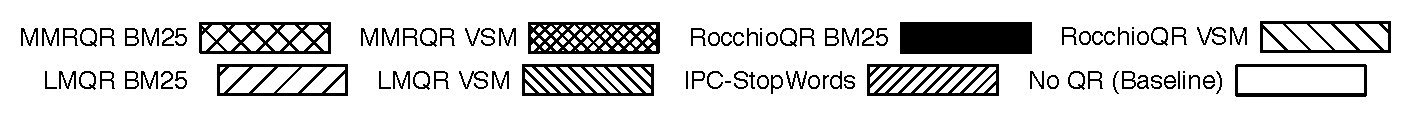
\includegraphics[width=9cm]{img/legendQR2}
\par\end{centering}

\begin{centering}
\subfigure[Q. Abstract.]{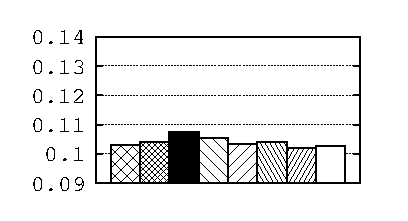
\includegraphics[width=3cm]{mmrqrResults/qAbstract-MAP-CLEF-IP2010}
}\subfigure[Q. Ext. Abstract.]{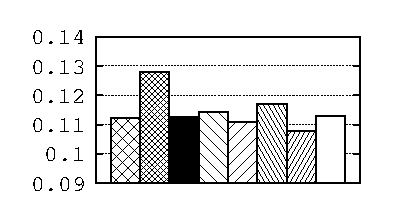
\includegraphics[width=3cm]{mmrqrResults/qExtAbstract-MAP-CLEF-IP2010}
}\subfigure[Q. Description.]{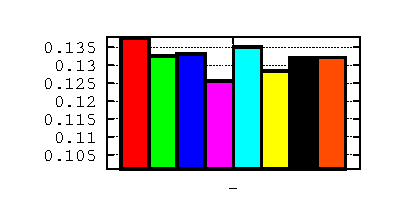
\includegraphics[width=3cm]{mmrqrResults/qDescription-MAP-CLEF-IP2010}
}
\par\end{centering}

\protect\caption{MAP for QR methods on CLEF-IP 2010.}


\label{fig:QR-MAP-CLEF-IP2010} 
\end{figure}

\par\end{center}

\begin{center}
\begin{figure}
\begin{centering}
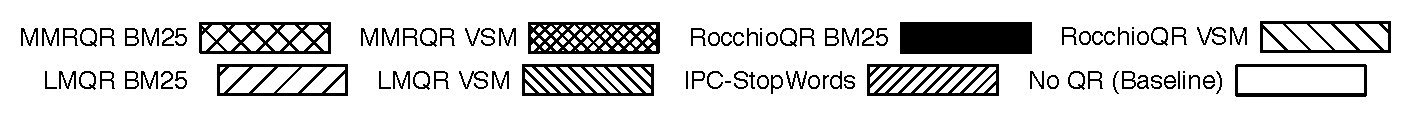
\includegraphics[width=9cm]{img/legendQR2} 
\par\end{centering}

\begin{centering}
\subfigure[Q. Abstract.]{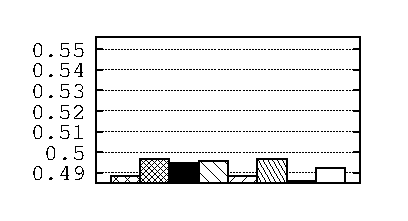
\includegraphics[width=3cm]{mmrqrResults/qAbstract-PRES-CLEF-IP2010}
}\subfigure[Q. Ext. Abstract.]{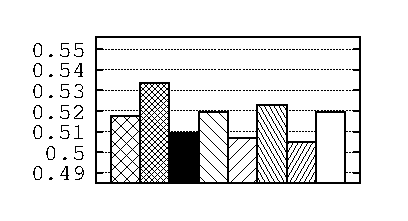
\includegraphics[width=3cm]{mmrqrResults/qExtAbstract-PRES-CLEF-IP2010}
}\subfigure[Q. Description.]{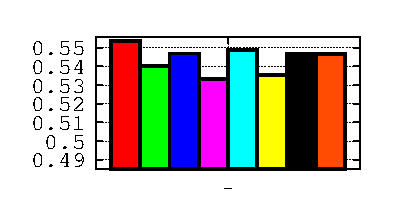
\includegraphics[width=3cm]{mmrqrResults/qDescription-PRES-CLEF-IP2010}
}
\par\end{centering}

\protect\protect\caption{PRES for QR methods on CLEF 2010.}


\label{fig:QR-PRES-CLEF-IP2010} 
\end{figure}

\par\end{center}

Finally, to give an insight of the effect of MMRQR and LMQR over the
performance, Table \ref{tbl:QRSampleQueries} shows some queries where
QR methods are helpful. Terms in bold are terms removed by MMRQR,
whereas terms underlined are terms removed by Rocchio. Terms removed
by the two methods are both in bold and underlined. First, we notice
that even when there are common terms removed from the original queries
by both MMRQR and LMQR, the terms removed by MMRQR tend to be similar
between them (e.g., \textit{laser, light, interferometer}, in 1-Topic),
which favor retaining diverse relevant terms in the query. However,
for the third topic, MMRQR removed the main terms from the query (\textit{motor},
and thermal \textit{load}), which probably decreases the quality of
the query.


\section{Related work}

\label{sec:RelatedWork}

We believe the outlined patent-specific query reformulation methods
described in Section \ref{sec:QueryReformulation} circumscribe a
range of patent-specific approaches spanning synonym lexicons, specially
derived language models, and IPC code resources; hence our evaluation
supported the objective of identifying general query reformulation
methods from the novel perspective of partial patent application prior
art search that may be deserving of further investigation in future
work.

However, some more complex patent-specific methods have also been
explored for general patent prior art search. The scenario of patent
prior art search consists of manually forming queries by selecting
high frequency terms from patent application. Hence, in \cite{Itoh2003},
authors proposed a new term selection method using different term
frequencies depending on the genre in the NTCIR-3 Patent Retrieval
Task.

\begin{center}
\begin{figure}[t]
\begin{centering}
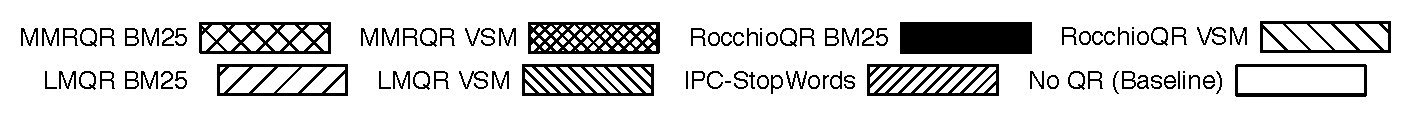
\includegraphics[width=9cm]{img/legendQR2}
\par\end{centering}

\begin{centering}
\subfigure[Q. Abstract.]{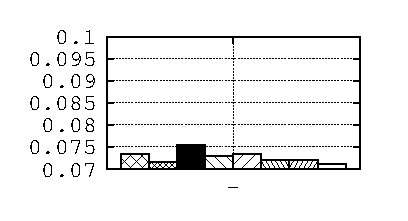
\includegraphics[width=3cm]{mmrqrResults/qAbstract-MAP-CLEF-IP2011}
}\subfigure[Q. Ext. Abstract.]{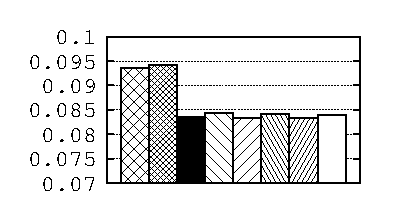
\includegraphics[width=3cm]{mmrqrResults/qExtAbstract-MAP-CLEF-IP2011}
}\subfigure[Q. Description.]{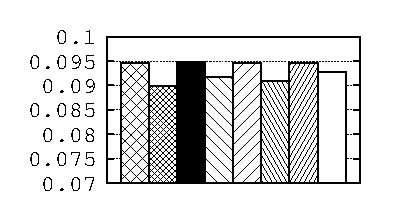
\includegraphics[width=3cm]{mmrqrResults/qDescription-MAP-CLEF-IP2011}
}
\par\end{centering}

\protect\caption{MAP for QR methods on CLEF-IP 2011.}


\label{fig:QR-MAP-CLEF-IP2011} 
\end{figure}

\par\end{center}

\begin{center}
\begin{figure}
\begin{centering}
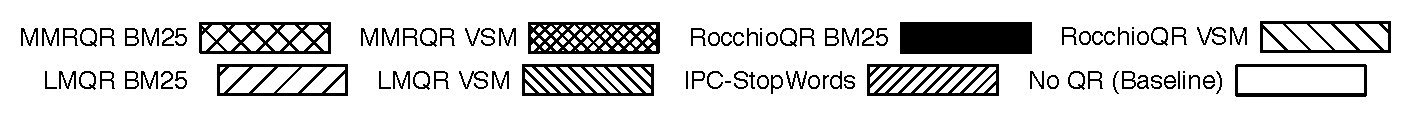
\includegraphics[width=9cm]{img/legendQR2}
\par\end{centering}

\begin{centering}
\subfigure[Q. Abstract.]{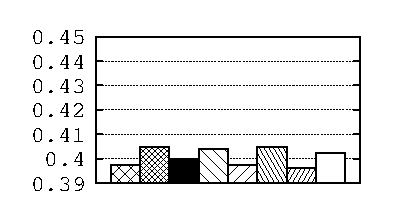
\includegraphics[width=3cm]{mmrqrResults/qAbstract-PRES-CLEF-IP2011}
}\subfigure[Q. Ext. Abstract.]{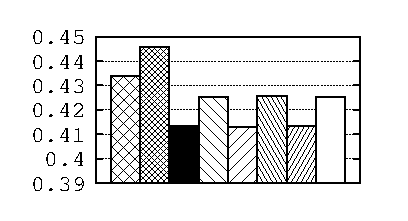
\includegraphics[width=3cm]{mmrqrResults/qExtAbstract-PRES-CLEF-IP2011}
}\subfigure[Q. Description.]{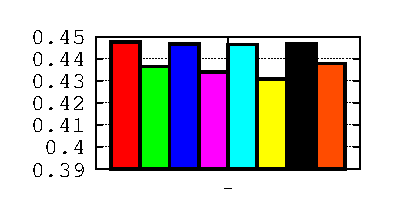
\includegraphics[width=3cm]{mmrqrResults/qDescription-PRES-CLEF-IP2011}
}
\par\end{centering}

\protect\protect\caption{PRES for QR methods on CLEF 2011.}


\label{fig:QR-PRES-CLEF-IP2011} 
\end{figure}

\par\end{center}

Also, Xue and Croft \cite{Xue:2009:TPP:1571941.1572139} advocates
the use of the full patent application as the query to reduce the
burden on patent examiners. They conducted a series of experiments
in order to examine the effect of different patent fields, and concludes
with the observation that the best Mean Average Precision (MAP) is
achieved using the text from the description section of the query
patent with raw term frequencies. Also, Fuji \cite{Fujii:2007:EPR:1277741.1277912}
showed that retrieval effectiveness can be improved by combining IR
methods with the result of citation extraction.

\begin{center}
\begin{table*}[t]
\protect\caption{Samples of queries extracted from CLEF-IP 2011, where MMRQR improves
the performance. (P: Precision, R: Recall, RR: Reciprocal Rank, AP:
Average Precision, PRES: Patent Retrieval Evaluation Score). MMRQR
improves the two first examples, while LMQR improves the third. }
\label{tbl:QRSampleQueries}

\centering{}%
\begin{tabular}{|>{\raggedright}p{17.5cm}|}
\hline 
\textbf{\scriptsize{}1- Topic: }{\scriptsize{}EP-1424597-A2}\tabularnewline
\hline 
\textbf{\scriptsize{}Abstract:}{\scriptsize{} Measurements of an interferometric
measurement system are corrected for variations of atmospheric conditions
such as pressure, temperature and turbulence using measurements from
a second harmonic interferometer (10). A ramp, representing the dependence
of the SHI data on path length, is removed before use of the SHI data.
The SHI may use a passive Q-switched laser (11) as a light source
and Brewster prisms (142,144) in the receiver module. Optical fibers
may be used to conduct light to the detectors (145-147). A mirror
reflecting the measurement beams has a coating of a thickness selected
to minimize the sensitivity of the SHI data to changes in coating
thickness.}\tabularnewline
\hline 
\begin{tabular}{>{\centering}p{16.5cm}}
{\scriptsize{}Baseline performance:}~{\scriptsize{}}%
\begin{tabular}{|c|c|c|c|c|c|c|c|c|c|c|c|}
\hline 
\textbf{\scriptsize{}P@5:} & {\scriptsize{}0.000} & \textbf{\scriptsize{}P@10:} & {\scriptsize{}0.000} & \textbf{\scriptsize{}R@10:} & {\scriptsize{}0.000} & \textbf{\scriptsize{}RR:} & {\scriptsize{}0.037} & \textbf{\scriptsize{}AP:} & {\scriptsize{}0.022} & \textbf{\scriptsize{}PRES:} & {\scriptsize{}0.648}\tabularnewline
\hline 
\end{tabular}\tabularnewline
\end{tabular}\tabularnewline
\hline 
\textbf{\scriptsize{}MMRQR removed terms: temperatur}{\scriptsize{},
}\textbf{\scriptsize{}detector}{\scriptsize{}, }\textbf{\scriptsize{}path}{\scriptsize{},
}\textbf{\scriptsize{}laser}{\scriptsize{}, }\textbf{\scriptsize{}light}{\scriptsize{},
}\textbf{\scriptsize{}interferometr}{\scriptsize{}, }\textbf{\scriptsize{}brewster}{\scriptsize{},
}\textbf{\scriptsize{}sensit}{\scriptsize{}, }\textbf{\scriptsize{}repres}{\scriptsize{},
}\textbf{\scriptsize{}sourc}\tabularnewline
\hline 
\begin{tabular}{>{\centering}p{16.5cm}}
{\scriptsize{}MMRQR performance:}~{\scriptsize{}}%
\begin{tabular}{|c|c|c|c|c|c|c|c|c|c|c|c|}
\hline 
\textbf{\scriptsize{}P@5:} & {\scriptsize{}0.000} & \textbf{\scriptsize{}P@10:} & {\scriptsize{}0.100} & \textbf{\scriptsize{}R@10:} & {\scriptsize{}0.166} & \textbf{\scriptsize{}RR:} & {\scriptsize{}0.111} & \textbf{\scriptsize{}AP:} & {\scriptsize{}0.053} & \textbf{\scriptsize{}PRES:} & {\scriptsize{}0.761}\tabularnewline
\hline 
\end{tabular}\tabularnewline
\end{tabular}\tabularnewline
\hline 
\textbf{\scriptsize{}LMQR removed terms: }{\scriptsize{}\uline{minim}}{\scriptsize{},
}{\scriptsize{}\uline{conduct}}{\scriptsize{}, }{\scriptsize{}\uline{variat}}{\scriptsize{},
}{\scriptsize{}\uline{shi}}{\scriptsize{}, }{\scriptsize{}\uline{turbul}}{\scriptsize{},
}{\scriptsize{}\uline{condit}}{\scriptsize{}, }{\scriptsize{}\uline{pressur}}{\scriptsize{},
}{\scriptsize{}\uline{remov}}{\scriptsize{}, }{\scriptsize{}\uline{ramp}}{\scriptsize{},
}{\scriptsize{}\uline{thick}}\tabularnewline
\hline 
\begin{tabular}{>{\centering}p{16.5cm}}
{\scriptsize{}LMQR performance:}~{\scriptsize{}}%
\begin{tabular}{|c|c|c|c|c|c|c|c|c|c|c|c|}
\hline 
\textbf{\scriptsize{}P@5:} & {\scriptsize{}0.000} & \textbf{\scriptsize{}P@10:} & {\scriptsize{}0.000} & \textbf{\scriptsize{}R@10:} & {\scriptsize{}0.000} & \textbf{\scriptsize{}RR:} & {\scriptsize{}0.076} & \textbf{\scriptsize{}AP:} & {\scriptsize{}0.036} & \textbf{\scriptsize{}PRES:} & {\scriptsize{}0.724}\tabularnewline
\hline 
\end{tabular}\tabularnewline
\end{tabular}\tabularnewline
\hline 
\hline 
\textbf{\scriptsize{}2- Topic: }{\scriptsize{}EP-1498393-A1}\tabularnewline
\hline 
\textbf{\scriptsize{}Abstract:}{\scriptsize{} In methods for recovering
and recycling helium and unreacted chlorine from a process for manufacturing
optical fiber an exhaust gas is recovered typically from a consolidation
furnace and is separated into helium-rich and chlorine-rich gas streams.
The helium-rich stream is typically dried and blended with make-up
helium and the chlorine-rich stream is typically purified and blended
with make-up chlorine so that both may be reused in the optical fiber
production process.}\tabularnewline
\hline 
\begin{tabular}{>{\centering}p{16.5cm}}
{\scriptsize{}Baseline performance:}~{\scriptsize{}}%
\begin{tabular}{|c|c|c|c|c|c|c|c|c|c|c|c|}
\hline 
\textbf{\scriptsize{}P@5:} & {\scriptsize{}0.200} & \textbf{\scriptsize{}P@10:} & {\scriptsize{}0.100} & \textbf{\scriptsize{}R@10:} & {\scriptsize{}0.125} & \textbf{\scriptsize{}RR:} & {\scriptsize{}0.200} & \textbf{\scriptsize{}AP:} & {\scriptsize{}0.060} & \textbf{\scriptsize{}PRES:} & {\scriptsize{}0.481}\tabularnewline
\hline 
\end{tabular}\tabularnewline
\end{tabular}\tabularnewline
\hline 
\textbf{\scriptsize{}MMRQR removed terms: stream}{\scriptsize{}, }\textbf{\scriptsize{}\uline{rich}}{\scriptsize{},
}\textbf{\scriptsize{}fiber}{\scriptsize{}, }\textbf{\scriptsize{}\uline{reus}}{\scriptsize{},
}\textbf{\scriptsize{}\uline{product}}{\scriptsize{}, }\textbf{\scriptsize{}\uline{dri}}{\scriptsize{},
}\textbf{\scriptsize{}separ}{\scriptsize{}, }\textbf{\scriptsize{}exhaust}{\scriptsize{},
}\textbf{\scriptsize{}\uline{method}}{\scriptsize{}, }\textbf{\scriptsize{}\uline{make}}\tabularnewline
\hline 
\begin{tabular}{>{\centering}p{16.5cm}}
{\scriptsize{}MMRQR performance:}~{\scriptsize{}}%
\begin{tabular}{|c|c|c|c|c|c|c|c|c|c|c|c|}
\hline 
\textbf{\scriptsize{}P@5:} & {\scriptsize{}0.200} & \textbf{\scriptsize{}P@10:} & {\scriptsize{}0.200} & \textbf{\scriptsize{}R@10:} & {\scriptsize{}0.250} & \textbf{\scriptsize{}RR:} & {\scriptsize{}0.250} & \textbf{\scriptsize{}AP:} & {\scriptsize{}0.106} & \textbf{\scriptsize{}PRES:} & {\scriptsize{}0.604}\tabularnewline
\hline 
\end{tabular}\tabularnewline
\end{tabular}\tabularnewline
\hline 
\textbf{\scriptsize{}LMQR removed terms: }\textbf{\scriptsize{}\uline{dri}}{\scriptsize{},
}\textbf{\scriptsize{}\uline{rich}}{\scriptsize{}, }{\scriptsize{}\uline{process}}{\scriptsize{},
}\textbf{\scriptsize{}\uline{product}}{\scriptsize{}, }\textbf{\scriptsize{}\uline{make}}{\scriptsize{},
}\textbf{\scriptsize{}\uline{reus}}{\scriptsize{}, }{\scriptsize{}\uline{unreact}}{\scriptsize{},
}{\scriptsize{}\uline{typic}}{\scriptsize{}, }{\scriptsize{}\uline{blend}}{\scriptsize{},
}\textbf{\scriptsize{}\uline{method}}{\scriptsize{}, }\tabularnewline
\hline 
\begin{tabular}{>{\centering}p{16.5cm}}
{\scriptsize{}LMQR performance:}~{\scriptsize{}}%
\begin{tabular}{|c|c|c|c|c|c|c|c|c|c|c|c|}
\hline 
\textbf{\scriptsize{}P@5:} & {\scriptsize{}0.200} & \textbf{\scriptsize{}P@10:} & {\scriptsize{}0.200} & \textbf{\scriptsize{}R@10:} & {\scriptsize{}0.250} & \textbf{\scriptsize{}RR:} & {\scriptsize{}0.200} & \textbf{\scriptsize{}AP:} & {\scriptsize{}0.097} & \textbf{\scriptsize{}PRES:} & {\scriptsize{}0.552}\tabularnewline
\hline 
\end{tabular}\tabularnewline
\end{tabular}\tabularnewline
\hline 
\hline 
\textbf{\scriptsize{}3- Topic: }{\scriptsize{}EP-1314594-A1}\tabularnewline
\hline 
\textbf{\scriptsize{}Abstract:}{\scriptsize{} An air conditioner for
air conditioning the interior of a compartment includes a compressor
(C) and an electric motor (84). The compressor (C) compresses refrigerant
gas and changes the displacement. The electric motor (84) drives the
compressor (C). A motor controller (72) rotates the motor (84) at
a constant reference speed. A detection device (92) detects information
related to the thermal load on the air conditioner. A current sensor
(97) detects the value of current supplied to the electric motor.
A controller (72) controls the compressor based on the detected thermal
load information and the detected current value. The controller (72)
computes a target torque of the compressor based on the thermal load
information. In accordance with the computed target torque, the controller
(72) computes a target current value to be supplied to the electric
motor. The controller (72) further controls the displacement of the
compressor such that the detected current value matches the target
current value.}\tabularnewline
\hline 
\begin{tabular}{>{\centering}p{16.5cm}}
{\scriptsize{}Baseline performance:}~{\scriptsize{}}%
\begin{tabular}{|c|c|c|c|c|c|c|c|c|c|c|c|}
\hline 
\textbf{\scriptsize{}P@5:} & {\scriptsize{}0.600} & \textbf{\scriptsize{}P@10:} & {\scriptsize{}0.400} & \textbf{\scriptsize{}R@10:} & {\scriptsize{}0.307} & \textbf{\scriptsize{}RR:} & {\scriptsize{}1.000} & \textbf{\scriptsize{}AP:} & {\scriptsize{}0.301} & \textbf{\scriptsize{}PRES:} & {\scriptsize{}0.777}\tabularnewline
\hline 
\end{tabular}\tabularnewline
\end{tabular}\tabularnewline
\hline 
\textbf{\scriptsize{}MMRQR removed terms:}{\scriptsize{} }\textbf{\scriptsize{}\uline{refer}}{\scriptsize{},
}\textbf{\scriptsize{}motor}{\scriptsize{}, }\textbf{\scriptsize{}\uline{current}}{\scriptsize{},
}\textbf{\scriptsize{}\uline{relat}}{\scriptsize{}, }\textbf{\scriptsize{}condit}{\scriptsize{},
}\textbf{\scriptsize{}constant}{\scriptsize{}, }\textbf{\scriptsize{}\uline{suppli}}{\scriptsize{},
}\textbf{\scriptsize{}\uline{compress}}{\scriptsize{}, }\textbf{\scriptsize{}load}{\scriptsize{},
}\textbf{\scriptsize{}\uline{match}}\tabularnewline
\hline 
\begin{tabular}{>{\centering}p{16.5cm}}
{\scriptsize{}MMRQR performance:}~{\scriptsize{}}%
\begin{tabular}{|c|c|c|c|c|c|c|c|c|c|c|c|}
\hline 
\textbf{\scriptsize{}P@5:} & {\scriptsize{}0.400} & \textbf{\scriptsize{}P@10:} & {\scriptsize{}0.500} & \textbf{\scriptsize{}R@10:} & {\scriptsize{}0.384} & \textbf{\scriptsize{}RR}{\scriptsize{}:} & {\scriptsize{}0.500} & \textbf{\scriptsize{}AP:} & {\scriptsize{}0.221} & \textbf{\scriptsize{}PRES:} & {\scriptsize{}0.774}\tabularnewline
\hline 
\end{tabular}\tabularnewline
\end{tabular}\tabularnewline
\hline 
\textbf{\scriptsize{}LMQR removed terms: }{\scriptsize{}\uline{compart}}{\scriptsize{},
}\textbf{\scriptsize{}\uline{suppli}}{\scriptsize{}, }\textbf{\scriptsize{}\uline{current}}{\scriptsize{},
}{\scriptsize{}\uline{ga}}{\scriptsize{}, }\textbf{\scriptsize{}\uline{refer}}{\scriptsize{},
}\textbf{\scriptsize{}\uline{compress}}{\scriptsize{}, }\textbf{\scriptsize{}\uline{relat}}{\scriptsize{},
}{\scriptsize{}\uline{interior}}{\scriptsize{}, }{\scriptsize{}\uline{thermal}}{\scriptsize{},
}\textbf{\scriptsize{}\uline{match}}{\scriptsize{}, }\tabularnewline
\hline 
\begin{tabular}{>{\centering}p{16.5cm}}
{\scriptsize{}LMQR performance:}~{\scriptsize{}}%
\begin{tabular}{|c|c|c|c|c|c|c|c|c|c|c|c|}
\hline 
\textbf{\scriptsize{}P@5:} & {\scriptsize{}0.400} & \textbf{\scriptsize{}P@10:} & {\scriptsize{}0.400} & \textbf{\scriptsize{}R@10:} & {\scriptsize{}0.307} & \textbf{\scriptsize{}RR:} & {\scriptsize{}1.000} & \textbf{\scriptsize{}AP:} & {\scriptsize{}0.266} & \textbf{\scriptsize{}PRES:} & {\scriptsize{}0.802}\tabularnewline
\hline 
\end{tabular}\tabularnewline
\end{tabular}\tabularnewline
\hline 
\end{tabular}
\end{table*}

\par\end{center}

Bashir et al. \cite{Bashir2010} propose a query expansion with pseudo-relevance
feedback. Query expansion terms are selected using a using a machine
learning approach, by picking terms that may have a potential positive
impact on the retrieval effectiveness. However, this approach can
be computationally expensive, since the presented features are complicated
to compute, e.g. Pair-wise Terms Proximity features. Verma and Varma
\cite{Verma2011} propose a different approach, which instead of using
the patent text to query, use its International Patent Classification
(IPC) codes, which are expanded using the citation network. The formed
query is used to perform an initial search. The results are then re-ranked
using queries constructed from patent text. Throughout our experiments,
we concluded that relying on other terms to form a query rather than
those in the patent application, leads to poor retrieval quality.
Lastly, a more recent work by Mahdabi et al. \cite{Mahdabi:2014:PQF:2684820.2651363}
propose a unified framework for query expansion which incorporates
bibliographic information, IPC classifications, and temporal features
to improve the initial query built from the query patent. They used
the link-based structure of the citation graph together with the term
distribution of cited documents and built a query model from the citation
graph. They also used the publication dates associated with the patents
to adapt the query model to the change of vocabulary over time. The
results showed the advantage of using the term distribution of the
cited documents together with the publication dates. In \cite{Mahdabi:2014:ECA:2673721.2673730}
authors propose to build a topic dependent citation graph, starting
from the initially retrieved set of feedback documents and utilizing
citation links of feedback documents to expand the set. They identify
the important documents in the topic dependent citation graph using
a citation analysis measure. Then, they use the term distribution
of the documents in the citation graph to estimate a query model by
identifying the distinguishing terms. Then, they use these terms to
expand the original query. Finally, in \cite{Mahdabi:2014:QMC:2661829.2661899}
authors propose a method based on a random walk in a network of patent
citations, to find influential documents in the citation network of
a query patent, which can serve as candidates for drawing query terms
and bigrams for query refinement.

\begin{comment}
Finally, other works investigated query suggestion for patent prior
art search, which reflect real-life scenario of examiners, who form
reproducible boolean queries \cite{Adams2011,Azzopardi2010,Kim2011}.
\end{comment}


%we do%do not show comparisons with these methods here for the following reasons:%(i) their authors already pointed out their poor performance \cite{Mahdabi2013}; %(ii) as reflected in our existing experiments, patent-specific lexicons%have not tended to yield significantly better query reformulation results%in comparison to generic methods~\cite{Magdy2011,Verma2011}; and %(iii) the method is computational too expensive \cite{Bashir2010}.


\section{Conclusions}

\label{sec:Conclusion}

In this paper, we analyzed various query strategies of patent prior
art search with partial (incomplete) applications along with generic
and patent-specific query reformulation (expansion and reduction)
methods. Hence, in this scenario of partial patent application, we
considered only sections, which are more likely to be written by the
inventor (i.e., the title, the abstract, the description section,
and an extended abstract). We performed a comprehensive comparative
evaluation of these methods on the CLEF-IP patent corpus for prior
art search.

We showed that the description is the best partial application section
to query with, followed by the extended abstract, the abstract, and
lastly the title section. However, the largest boost in performance
(about 165\% for MAP) comes when switching from a title query to an
abstract query or extended abstract; smaller relative boosts are given
by querying instead with the full description (about 10\% to 30\%
for MAP). This is a critical insight since it is substantially easier
for the patent inventor to draft an abstract or an extended abstract
rather than a full patent description and in doing so, still manage
to retrieve the majority of prior art that would have been retrieved
with the full description.

We observed that query expansion (QE) methods are useful for short
to medium length queries (i.e., title, abstract, and extended abstract),
but useless for very long queries (i.e., the description section).
We also showed that the description section does not provide the best
source of expansion terms for QE, rather the claims or the abstract
tend to offer better candidate terms for QE. In the same vein, we
also found traditional IR methods like Rocchio or variations to work
just as well for QE (and generally better) in comparison with patent-specific
methods that used specialized expansion sources such as synonym lexicons
or IPC code definitions (at least for the methods that we evaluated).
For QE, future work should investigate how can we exploit patent-specific
meta-data such as inventor and citation networks to better exploit
specialized domains of discourse relevant to patent subfields.

Regarding query reduction (QR) methods, we showed these techniques
are generally most effective compared to QE for the extended abstract
and the description sections (the two longest sections used as a partial
application query). Albeit by a slim margin over No QR, the overall
best retrieval performance results in this work are achieved with
generic (non-patent specific) QR methods for description queries.
Future work may consist of exploiting query quality predictors to
identify useless terms in a query using machine learning methods.

%Finally, it is clear that for a patent examiner, using the description%section of a patent application with perhaps a QR method like MMRQR%or RocchioQR will help to find the most relevant documents (to invalidate%the application). However, for inventors, before investing too much%time in writing a full patent application, we believe that it is better%to first write the abstract. Then, use Rocchio with expanded terms coming from%the claims to get the most relevant documents to make a prior art%search task (to position the current invention with related work).%These observations does not contradict with the  

In conclusion, we return to our initial objective to aid the patent
inventor in identifying an effective pre-application prior art search
strategy. Our evaluation reveals the critical insight that while querying
with a full description, perhaps combined with generic query reduction
methods, yields strong overall retrieval performance. Nonetheless,
we also find that querying with an abstract or an extended abstract
and using generic query reformulation methods represents the best
trade-off in terms of writing effort vs. retrieval efficacy (i.e.,
querying with the description sections only lead to marginal improvements).

Finally, we believe that future work should investigate whether QE
methods for abstract or extended abstract queries can rival the best
methods for description queries --- if such a result were possible,
it would significantly reduce the effort required on behalf of the
patent inventor to identify potentially invalidating prior art for
a new patent idea.

{\scriptsize

\bibliographystyle{abbrv}
\bibliography{biblio}


}
\end{document}
